\documentclass[11pt]{article}

    \usepackage[breakable]{tcolorbox}
    \usepackage{parskip} % Stop auto-indenting (to mimic markdown behaviour)
    
    \usepackage{iftex}
    \ifPDFTeX
    	\usepackage[T1]{fontenc}
    	\usepackage{mathpazo}
    \else
    	\usepackage{fontspec}
    \fi

    % Basic figure setup, for now with no caption control since it's done
    % automatically by Pandoc (which extracts ![](path) syntax from Markdown).
    \usepackage{graphicx}
    % Maintain compatibility with old templates. Remove in nbconvert 6.0
    \let\Oldincludegraphics\includegraphics
    % Ensure that by default, figures have no caption (until we provide a
    % proper Figure object with a Caption API and a way to capture that
    % in the conversion process - todo).
    \usepackage{caption}
    \DeclareCaptionFormat{nocaption}{}
    \captionsetup{format=nocaption,aboveskip=0pt,belowskip=0pt}

    \usepackage[Export]{adjustbox} % Used to constrain images to a maximum size
    \adjustboxset{max size={0.9\linewidth}{0.9\paperheight}}
    \usepackage{float}
    \floatplacement{figure}{H} % forces figures to be placed at the correct location
    \usepackage{xcolor} % Allow colors to be defined
    \usepackage{enumerate} % Needed for markdown enumerations to work
    \usepackage{geometry} % Used to adjust the document margins
    \usepackage{amsmath} % Equations
    \usepackage{amssymb} % Equations
    \usepackage{textcomp} % defines textquotesingle
    % Hack from http://tex.stackexchange.com/a/47451/13684:
    \AtBeginDocument{%
        \def\PYZsq{\textquotesingle}% Upright quotes in Pygmentized code
    }
    \usepackage{upquote} % Upright quotes for verbatim code
    \usepackage{eurosym} % defines \euro
    \usepackage[mathletters]{ucs} % Extended unicode (utf-8) support
    \usepackage{fancyvrb} % verbatim replacement that allows latex
    \usepackage{grffile} % extends the file name processing of package graphics 
                         % to support a larger range
    \makeatletter % fix for grffile with XeLaTeX
    \def\Gread@@xetex#1{%
      \IfFileExists{"\Gin@base".bb}%
      {\Gread@eps{\Gin@base.bb}}%
      {\Gread@@xetex@aux#1}%
    }
    \makeatother

    % The hyperref package gives us a pdf with properly built
    % internal navigation ('pdf bookmarks' for the table of contents,
    % internal cross-reference links, web links for URLs, etc.)
    \usepackage{hyperref}
    % The default LaTeX title has an obnoxious amount of whitespace. By default,
    % titling removes some of it. It also provides customization options.
    \usepackage{titling}
    \usepackage{longtable} % longtable support required by pandoc >1.10
    \usepackage{booktabs}  % table support for pandoc > 1.12.2
    \usepackage[inline]{enumitem} % IRkernel/repr support (it uses the enumerate* environment)
    \usepackage[normalem]{ulem} % ulem is needed to support strikethroughs (\sout)
                                % normalem makes italics be italics, not underlines
    \usepackage{mathrsfs}
    

    
    % Colors for the hyperref package
    \definecolor{urlcolor}{rgb}{0,.145,.698}
    \definecolor{linkcolor}{rgb}{.71,0.21,0.01}
    \definecolor{citecolor}{rgb}{.12,.54,.11}

    % ANSI colors
    \definecolor{ansi-black}{HTML}{3E424D}
    \definecolor{ansi-black-intense}{HTML}{282C36}
    \definecolor{ansi-red}{HTML}{E75C58}
    \definecolor{ansi-red-intense}{HTML}{B22B31}
    \definecolor{ansi-green}{HTML}{00A250}
    \definecolor{ansi-green-intense}{HTML}{007427}
    \definecolor{ansi-yellow}{HTML}{DDB62B}
    \definecolor{ansi-yellow-intense}{HTML}{B27D12}
    \definecolor{ansi-blue}{HTML}{208FFB}
    \definecolor{ansi-blue-intense}{HTML}{0065CA}
    \definecolor{ansi-magenta}{HTML}{D160C4}
    \definecolor{ansi-magenta-intense}{HTML}{A03196}
    \definecolor{ansi-cyan}{HTML}{60C6C8}
    \definecolor{ansi-cyan-intense}{HTML}{258F8F}
    \definecolor{ansi-white}{HTML}{C5C1B4}
    \definecolor{ansi-white-intense}{HTML}{A1A6B2}
    \definecolor{ansi-default-inverse-fg}{HTML}{FFFFFF}
    \definecolor{ansi-default-inverse-bg}{HTML}{000000}

    % commands and environments needed by pandoc snippets
    % extracted from the output of `pandoc -s`
    \providecommand{\tightlist}{%
      \setlength{\itemsep}{0pt}\setlength{\parskip}{0pt}}
    \DefineVerbatimEnvironment{Highlighting}{Verbatim}{commandchars=\\\{\}}
    % Add ',fontsize=\small' for more characters per line
    \newenvironment{Shaded}{}{}
    \newcommand{\KeywordTok}[1]{\textcolor[rgb]{0.00,0.44,0.13}{\textbf{{#1}}}}
    \newcommand{\DataTypeTok}[1]{\textcolor[rgb]{0.56,0.13,0.00}{{#1}}}
    \newcommand{\DecValTok}[1]{\textcolor[rgb]{0.25,0.63,0.44}{{#1}}}
    \newcommand{\BaseNTok}[1]{\textcolor[rgb]{0.25,0.63,0.44}{{#1}}}
    \newcommand{\FloatTok}[1]{\textcolor[rgb]{0.25,0.63,0.44}{{#1}}}
    \newcommand{\CharTok}[1]{\textcolor[rgb]{0.25,0.44,0.63}{{#1}}}
    \newcommand{\StringTok}[1]{\textcolor[rgb]{0.25,0.44,0.63}{{#1}}}
    \newcommand{\CommentTok}[1]{\textcolor[rgb]{0.38,0.63,0.69}{\textit{{#1}}}}
    \newcommand{\OtherTok}[1]{\textcolor[rgb]{0.00,0.44,0.13}{{#1}}}
    \newcommand{\AlertTok}[1]{\textcolor[rgb]{1.00,0.00,0.00}{\textbf{{#1}}}}
    \newcommand{\FunctionTok}[1]{\textcolor[rgb]{0.02,0.16,0.49}{{#1}}}
    \newcommand{\RegionMarkerTok}[1]{{#1}}
    \newcommand{\ErrorTok}[1]{\textcolor[rgb]{1.00,0.00,0.00}{\textbf{{#1}}}}
    \newcommand{\NormalTok}[1]{{#1}}
    
    % Additional commands for more recent versions of Pandoc
    \newcommand{\ConstantTok}[1]{\textcolor[rgb]{0.53,0.00,0.00}{{#1}}}
    \newcommand{\SpecialCharTok}[1]{\textcolor[rgb]{0.25,0.44,0.63}{{#1}}}
    \newcommand{\VerbatimStringTok}[1]{\textcolor[rgb]{0.25,0.44,0.63}{{#1}}}
    \newcommand{\SpecialStringTok}[1]{\textcolor[rgb]{0.73,0.40,0.53}{{#1}}}
    \newcommand{\ImportTok}[1]{{#1}}
    \newcommand{\DocumentationTok}[1]{\textcolor[rgb]{0.73,0.13,0.13}{\textit{{#1}}}}
    \newcommand{\AnnotationTok}[1]{\textcolor[rgb]{0.38,0.63,0.69}{\textbf{\textit{{#1}}}}}
    \newcommand{\CommentVarTok}[1]{\textcolor[rgb]{0.38,0.63,0.69}{\textbf{\textit{{#1}}}}}
    \newcommand{\VariableTok}[1]{\textcolor[rgb]{0.10,0.09,0.49}{{#1}}}
    \newcommand{\ControlFlowTok}[1]{\textcolor[rgb]{0.00,0.44,0.13}{\textbf{{#1}}}}
    \newcommand{\OperatorTok}[1]{\textcolor[rgb]{0.40,0.40,0.40}{{#1}}}
    \newcommand{\BuiltInTok}[1]{{#1}}
    \newcommand{\ExtensionTok}[1]{{#1}}
    \newcommand{\PreprocessorTok}[1]{\textcolor[rgb]{0.74,0.48,0.00}{{#1}}}
    \newcommand{\AttributeTok}[1]{\textcolor[rgb]{0.49,0.56,0.16}{{#1}}}
    \newcommand{\InformationTok}[1]{\textcolor[rgb]{0.38,0.63,0.69}{\textbf{\textit{{#1}}}}}
    \newcommand{\WarningTok}[1]{\textcolor[rgb]{0.38,0.63,0.69}{\textbf{\textit{{#1}}}}}
    
    
    % Define a nice break command that doesn't care if a line doesn't already
    % exist.
    \def\br{\hspace*{\fill} \\* }
    % Math Jax compatibility definitions
    \def\gt{>}
    \def\lt{<}
    \let\Oldtex\TeX
    \let\Oldlatex\LaTeX
    \renewcommand{\TeX}{\textrm{\Oldtex}}
    \renewcommand{\LaTeX}{\textrm{\Oldlatex}}
    % Document parameters
    % Document title
    \title{Digitale Signalverarbeitung mit Python}
    
    
    
    
    
% Pygments definitions
\makeatletter
\def\PY@reset{\let\PY@it=\relax \let\PY@bf=\relax%
    \let\PY@ul=\relax \let\PY@tc=\relax%
    \let\PY@bc=\relax \let\PY@ff=\relax}
\def\PY@tok#1{\csname PY@tok@#1\endcsname}
\def\PY@toks#1+{\ifx\relax#1\empty\else%
    \PY@tok{#1}\expandafter\PY@toks\fi}
\def\PY@do#1{\PY@bc{\PY@tc{\PY@ul{%
    \PY@it{\PY@bf{\PY@ff{#1}}}}}}}
\def\PY#1#2{\PY@reset\PY@toks#1+\relax+\PY@do{#2}}

\expandafter\def\csname PY@tok@w\endcsname{\def\PY@tc##1{\textcolor[rgb]{0.73,0.73,0.73}{##1}}}
\expandafter\def\csname PY@tok@c\endcsname{\let\PY@it=\textit\def\PY@tc##1{\textcolor[rgb]{0.25,0.50,0.50}{##1}}}
\expandafter\def\csname PY@tok@cp\endcsname{\def\PY@tc##1{\textcolor[rgb]{0.74,0.48,0.00}{##1}}}
\expandafter\def\csname PY@tok@k\endcsname{\let\PY@bf=\textbf\def\PY@tc##1{\textcolor[rgb]{0.00,0.50,0.00}{##1}}}
\expandafter\def\csname PY@tok@kp\endcsname{\def\PY@tc##1{\textcolor[rgb]{0.00,0.50,0.00}{##1}}}
\expandafter\def\csname PY@tok@kt\endcsname{\def\PY@tc##1{\textcolor[rgb]{0.69,0.00,0.25}{##1}}}
\expandafter\def\csname PY@tok@o\endcsname{\def\PY@tc##1{\textcolor[rgb]{0.40,0.40,0.40}{##1}}}
\expandafter\def\csname PY@tok@ow\endcsname{\let\PY@bf=\textbf\def\PY@tc##1{\textcolor[rgb]{0.67,0.13,1.00}{##1}}}
\expandafter\def\csname PY@tok@nb\endcsname{\def\PY@tc##1{\textcolor[rgb]{0.00,0.50,0.00}{##1}}}
\expandafter\def\csname PY@tok@nf\endcsname{\def\PY@tc##1{\textcolor[rgb]{0.00,0.00,1.00}{##1}}}
\expandafter\def\csname PY@tok@nc\endcsname{\let\PY@bf=\textbf\def\PY@tc##1{\textcolor[rgb]{0.00,0.00,1.00}{##1}}}
\expandafter\def\csname PY@tok@nn\endcsname{\let\PY@bf=\textbf\def\PY@tc##1{\textcolor[rgb]{0.00,0.00,1.00}{##1}}}
\expandafter\def\csname PY@tok@ne\endcsname{\let\PY@bf=\textbf\def\PY@tc##1{\textcolor[rgb]{0.82,0.25,0.23}{##1}}}
\expandafter\def\csname PY@tok@nv\endcsname{\def\PY@tc##1{\textcolor[rgb]{0.10,0.09,0.49}{##1}}}
\expandafter\def\csname PY@tok@no\endcsname{\def\PY@tc##1{\textcolor[rgb]{0.53,0.00,0.00}{##1}}}
\expandafter\def\csname PY@tok@nl\endcsname{\def\PY@tc##1{\textcolor[rgb]{0.63,0.63,0.00}{##1}}}
\expandafter\def\csname PY@tok@ni\endcsname{\let\PY@bf=\textbf\def\PY@tc##1{\textcolor[rgb]{0.60,0.60,0.60}{##1}}}
\expandafter\def\csname PY@tok@na\endcsname{\def\PY@tc##1{\textcolor[rgb]{0.49,0.56,0.16}{##1}}}
\expandafter\def\csname PY@tok@nt\endcsname{\let\PY@bf=\textbf\def\PY@tc##1{\textcolor[rgb]{0.00,0.50,0.00}{##1}}}
\expandafter\def\csname PY@tok@nd\endcsname{\def\PY@tc##1{\textcolor[rgb]{0.67,0.13,1.00}{##1}}}
\expandafter\def\csname PY@tok@s\endcsname{\def\PY@tc##1{\textcolor[rgb]{0.73,0.13,0.13}{##1}}}
\expandafter\def\csname PY@tok@sd\endcsname{\let\PY@it=\textit\def\PY@tc##1{\textcolor[rgb]{0.73,0.13,0.13}{##1}}}
\expandafter\def\csname PY@tok@si\endcsname{\let\PY@bf=\textbf\def\PY@tc##1{\textcolor[rgb]{0.73,0.40,0.53}{##1}}}
\expandafter\def\csname PY@tok@se\endcsname{\let\PY@bf=\textbf\def\PY@tc##1{\textcolor[rgb]{0.73,0.40,0.13}{##1}}}
\expandafter\def\csname PY@tok@sr\endcsname{\def\PY@tc##1{\textcolor[rgb]{0.73,0.40,0.53}{##1}}}
\expandafter\def\csname PY@tok@ss\endcsname{\def\PY@tc##1{\textcolor[rgb]{0.10,0.09,0.49}{##1}}}
\expandafter\def\csname PY@tok@sx\endcsname{\def\PY@tc##1{\textcolor[rgb]{0.00,0.50,0.00}{##1}}}
\expandafter\def\csname PY@tok@m\endcsname{\def\PY@tc##1{\textcolor[rgb]{0.40,0.40,0.40}{##1}}}
\expandafter\def\csname PY@tok@gh\endcsname{\let\PY@bf=\textbf\def\PY@tc##1{\textcolor[rgb]{0.00,0.00,0.50}{##1}}}
\expandafter\def\csname PY@tok@gu\endcsname{\let\PY@bf=\textbf\def\PY@tc##1{\textcolor[rgb]{0.50,0.00,0.50}{##1}}}
\expandafter\def\csname PY@tok@gd\endcsname{\def\PY@tc##1{\textcolor[rgb]{0.63,0.00,0.00}{##1}}}
\expandafter\def\csname PY@tok@gi\endcsname{\def\PY@tc##1{\textcolor[rgb]{0.00,0.63,0.00}{##1}}}
\expandafter\def\csname PY@tok@gr\endcsname{\def\PY@tc##1{\textcolor[rgb]{1.00,0.00,0.00}{##1}}}
\expandafter\def\csname PY@tok@ge\endcsname{\let\PY@it=\textit}
\expandafter\def\csname PY@tok@gs\endcsname{\let\PY@bf=\textbf}
\expandafter\def\csname PY@tok@gp\endcsname{\let\PY@bf=\textbf\def\PY@tc##1{\textcolor[rgb]{0.00,0.00,0.50}{##1}}}
\expandafter\def\csname PY@tok@go\endcsname{\def\PY@tc##1{\textcolor[rgb]{0.53,0.53,0.53}{##1}}}
\expandafter\def\csname PY@tok@gt\endcsname{\def\PY@tc##1{\textcolor[rgb]{0.00,0.27,0.87}{##1}}}
\expandafter\def\csname PY@tok@err\endcsname{\def\PY@bc##1{\setlength{\fboxsep}{0pt}\fcolorbox[rgb]{1.00,0.00,0.00}{1,1,1}{\strut ##1}}}
\expandafter\def\csname PY@tok@kc\endcsname{\let\PY@bf=\textbf\def\PY@tc##1{\textcolor[rgb]{0.00,0.50,0.00}{##1}}}
\expandafter\def\csname PY@tok@kd\endcsname{\let\PY@bf=\textbf\def\PY@tc##1{\textcolor[rgb]{0.00,0.50,0.00}{##1}}}
\expandafter\def\csname PY@tok@kn\endcsname{\let\PY@bf=\textbf\def\PY@tc##1{\textcolor[rgb]{0.00,0.50,0.00}{##1}}}
\expandafter\def\csname PY@tok@kr\endcsname{\let\PY@bf=\textbf\def\PY@tc##1{\textcolor[rgb]{0.00,0.50,0.00}{##1}}}
\expandafter\def\csname PY@tok@bp\endcsname{\def\PY@tc##1{\textcolor[rgb]{0.00,0.50,0.00}{##1}}}
\expandafter\def\csname PY@tok@fm\endcsname{\def\PY@tc##1{\textcolor[rgb]{0.00,0.00,1.00}{##1}}}
\expandafter\def\csname PY@tok@vc\endcsname{\def\PY@tc##1{\textcolor[rgb]{0.10,0.09,0.49}{##1}}}
\expandafter\def\csname PY@tok@vg\endcsname{\def\PY@tc##1{\textcolor[rgb]{0.10,0.09,0.49}{##1}}}
\expandafter\def\csname PY@tok@vi\endcsname{\def\PY@tc##1{\textcolor[rgb]{0.10,0.09,0.49}{##1}}}
\expandafter\def\csname PY@tok@vm\endcsname{\def\PY@tc##1{\textcolor[rgb]{0.10,0.09,0.49}{##1}}}
\expandafter\def\csname PY@tok@sa\endcsname{\def\PY@tc##1{\textcolor[rgb]{0.73,0.13,0.13}{##1}}}
\expandafter\def\csname PY@tok@sb\endcsname{\def\PY@tc##1{\textcolor[rgb]{0.73,0.13,0.13}{##1}}}
\expandafter\def\csname PY@tok@sc\endcsname{\def\PY@tc##1{\textcolor[rgb]{0.73,0.13,0.13}{##1}}}
\expandafter\def\csname PY@tok@dl\endcsname{\def\PY@tc##1{\textcolor[rgb]{0.73,0.13,0.13}{##1}}}
\expandafter\def\csname PY@tok@s2\endcsname{\def\PY@tc##1{\textcolor[rgb]{0.73,0.13,0.13}{##1}}}
\expandafter\def\csname PY@tok@sh\endcsname{\def\PY@tc##1{\textcolor[rgb]{0.73,0.13,0.13}{##1}}}
\expandafter\def\csname PY@tok@s1\endcsname{\def\PY@tc##1{\textcolor[rgb]{0.73,0.13,0.13}{##1}}}
\expandafter\def\csname PY@tok@mb\endcsname{\def\PY@tc##1{\textcolor[rgb]{0.40,0.40,0.40}{##1}}}
\expandafter\def\csname PY@tok@mf\endcsname{\def\PY@tc##1{\textcolor[rgb]{0.40,0.40,0.40}{##1}}}
\expandafter\def\csname PY@tok@mh\endcsname{\def\PY@tc##1{\textcolor[rgb]{0.40,0.40,0.40}{##1}}}
\expandafter\def\csname PY@tok@mi\endcsname{\def\PY@tc##1{\textcolor[rgb]{0.40,0.40,0.40}{##1}}}
\expandafter\def\csname PY@tok@il\endcsname{\def\PY@tc##1{\textcolor[rgb]{0.40,0.40,0.40}{##1}}}
\expandafter\def\csname PY@tok@mo\endcsname{\def\PY@tc##1{\textcolor[rgb]{0.40,0.40,0.40}{##1}}}
\expandafter\def\csname PY@tok@ch\endcsname{\let\PY@it=\textit\def\PY@tc##1{\textcolor[rgb]{0.25,0.50,0.50}{##1}}}
\expandafter\def\csname PY@tok@cm\endcsname{\let\PY@it=\textit\def\PY@tc##1{\textcolor[rgb]{0.25,0.50,0.50}{##1}}}
\expandafter\def\csname PY@tok@cpf\endcsname{\let\PY@it=\textit\def\PY@tc##1{\textcolor[rgb]{0.25,0.50,0.50}{##1}}}
\expandafter\def\csname PY@tok@c1\endcsname{\let\PY@it=\textit\def\PY@tc##1{\textcolor[rgb]{0.25,0.50,0.50}{##1}}}
\expandafter\def\csname PY@tok@cs\endcsname{\let\PY@it=\textit\def\PY@tc##1{\textcolor[rgb]{0.25,0.50,0.50}{##1}}}

\def\PYZbs{\char`\\}
\def\PYZus{\char`\_}
\def\PYZob{\char`\{}
\def\PYZcb{\char`\}}
\def\PYZca{\char`\^}
\def\PYZam{\char`\&}
\def\PYZlt{\char`\<}
\def\PYZgt{\char`\>}
\def\PYZsh{\char`\#}
\def\PYZpc{\char`\%}
\def\PYZdl{\char`\$}
\def\PYZhy{\char`\-}
\def\PYZsq{\char`\'}
\def\PYZdq{\char`\"}
\def\PYZti{\char`\~}
% for compatibility with earlier versions
\def\PYZat{@}
\def\PYZlb{[}
\def\PYZrb{]}
\makeatother


    % For linebreaks inside Verbatim environment from package fancyvrb. 
    \makeatletter
        \newbox\Wrappedcontinuationbox 
        \newbox\Wrappedvisiblespacebox 
        \newcommand*\Wrappedvisiblespace {\textcolor{red}{\textvisiblespace}} 
        \newcommand*\Wrappedcontinuationsymbol {\textcolor{red}{\llap{\tiny$\m@th\hookrightarrow$}}} 
        \newcommand*\Wrappedcontinuationindent {3ex } 
        \newcommand*\Wrappedafterbreak {\kern\Wrappedcontinuationindent\copy\Wrappedcontinuationbox} 
        % Take advantage of the already applied Pygments mark-up to insert 
        % potential linebreaks for TeX processing. 
        %        {, <, #, %, $, ' and ": go to next line. 
        %        _, }, ^, &, >, - and ~: stay at end of broken line. 
        % Use of \textquotesingle for straight quote. 
        \newcommand*\Wrappedbreaksatspecials {% 
            \def\PYGZus{\discretionary{\char`\_}{\Wrappedafterbreak}{\char`\_}}% 
            \def\PYGZob{\discretionary{}{\Wrappedafterbreak\char`\{}{\char`\{}}% 
            \def\PYGZcb{\discretionary{\char`\}}{\Wrappedafterbreak}{\char`\}}}% 
            \def\PYGZca{\discretionary{\char`\^}{\Wrappedafterbreak}{\char`\^}}% 
            \def\PYGZam{\discretionary{\char`\&}{\Wrappedafterbreak}{\char`\&}}% 
            \def\PYGZlt{\discretionary{}{\Wrappedafterbreak\char`\<}{\char`\<}}% 
            \def\PYGZgt{\discretionary{\char`\>}{\Wrappedafterbreak}{\char`\>}}% 
            \def\PYGZsh{\discretionary{}{\Wrappedafterbreak\char`\#}{\char`\#}}% 
            \def\PYGZpc{\discretionary{}{\Wrappedafterbreak\char`\%}{\char`\%}}% 
            \def\PYGZdl{\discretionary{}{\Wrappedafterbreak\char`\$}{\char`\$}}% 
            \def\PYGZhy{\discretionary{\char`\-}{\Wrappedafterbreak}{\char`\-}}% 
            \def\PYGZsq{\discretionary{}{\Wrappedafterbreak\textquotesingle}{\textquotesingle}}% 
            \def\PYGZdq{\discretionary{}{\Wrappedafterbreak\char`\"}{\char`\"}}% 
            \def\PYGZti{\discretionary{\char`\~}{\Wrappedafterbreak}{\char`\~}}% 
        } 
        % Some characters . , ; ? ! / are not pygmentized. 
        % This macro makes them "active" and they will insert potential linebreaks 
        \newcommand*\Wrappedbreaksatpunct {% 
            \lccode`\~`\.\lowercase{\def~}{\discretionary{\hbox{\char`\.}}{\Wrappedafterbreak}{\hbox{\char`\.}}}% 
            \lccode`\~`\,\lowercase{\def~}{\discretionary{\hbox{\char`\,}}{\Wrappedafterbreak}{\hbox{\char`\,}}}% 
            \lccode`\~`\;\lowercase{\def~}{\discretionary{\hbox{\char`\;}}{\Wrappedafterbreak}{\hbox{\char`\;}}}% 
            \lccode`\~`\:\lowercase{\def~}{\discretionary{\hbox{\char`\:}}{\Wrappedafterbreak}{\hbox{\char`\:}}}% 
            \lccode`\~`\?\lowercase{\def~}{\discretionary{\hbox{\char`\?}}{\Wrappedafterbreak}{\hbox{\char`\?}}}% 
            \lccode`\~`\!\lowercase{\def~}{\discretionary{\hbox{\char`\!}}{\Wrappedafterbreak}{\hbox{\char`\!}}}% 
            \lccode`\~`\/\lowercase{\def~}{\discretionary{\hbox{\char`\/}}{\Wrappedafterbreak}{\hbox{\char`\/}}}% 
            \catcode`\.\active
            \catcode`\,\active 
            \catcode`\;\active
            \catcode`\:\active
            \catcode`\?\active
            \catcode`\!\active
            \catcode`\/\active 
            \lccode`\~`\~ 	
        }
    \makeatother

    \let\OriginalVerbatim=\Verbatim
    \makeatletter
    \renewcommand{\Verbatim}[1][1]{%
        %\parskip\z@skip
        \sbox\Wrappedcontinuationbox {\Wrappedcontinuationsymbol}%
        \sbox\Wrappedvisiblespacebox {\FV@SetupFont\Wrappedvisiblespace}%
        \def\FancyVerbFormatLine ##1{\hsize\linewidth
            \vtop{\raggedright\hyphenpenalty\z@\exhyphenpenalty\z@
                \doublehyphendemerits\z@\finalhyphendemerits\z@
                \strut ##1\strut}%
        }%
        % If the linebreak is at a space, the latter will be displayed as visible
        % space at end of first line, and a continuation symbol starts next line.
        % Stretch/shrink are however usually zero for typewriter font.
        \def\FV@Space {%
            \nobreak\hskip\z@ plus\fontdimen3\font minus\fontdimen4\font
            \discretionary{\copy\Wrappedvisiblespacebox}{\Wrappedafterbreak}
            {\kern\fontdimen2\font}%
        }%
        
        % Allow breaks at special characters using \PYG... macros.
        \Wrappedbreaksatspecials
        % Breaks at punctuation characters . , ; ? ! and / need catcode=\active 	
        \OriginalVerbatim[#1,codes*=\Wrappedbreaksatpunct]%
    }
    \makeatother

    % Exact colors from NB
    \definecolor{incolor}{HTML}{303F9F}
    \definecolor{outcolor}{HTML}{D84315}
    \definecolor{cellborder}{HTML}{CFCFCF}
    \definecolor{cellbackground}{HTML}{F7F7F7}
    
    % prompt
    \makeatletter
    \newcommand{\boxspacing}{\kern\kvtcb@left@rule\kern\kvtcb@boxsep}
    \makeatother
    \newcommand{\prompt}[4]{
        \ttfamily\llap{{\color{#2}[#3]:\hspace{3pt}#4}}\vspace{-\baselineskip}
    }
    

    
    % Prevent overflowing lines due to hard-to-break entities
    \sloppy 
    % Setup hyperref package
    \hypersetup{
      breaklinks=true,  % so long urls are correctly broken across lines
      colorlinks=true,
      urlcolor=urlcolor,
      linkcolor=linkcolor,
      citecolor=citecolor,
      }
    % Slightly bigger margins than the latex defaults
    
    \geometry{verbose,tmargin=1in,bmargin=1in,lmargin=1in,rmargin=1in}
    
    

\begin{document}
    
    \maketitle
    
    

    
    Autoren: Tashin Talbot, Thomas Radzieda, Peter Hanne

\hypertarget{digitale-signalverarbeitung-mit-python}{%
\section{Digitale signalverarbeitung mit
Python}\label{digitale-signalverarbeitung-mit-python}}

\hypertarget{einfuxfchrung}{%
\subsection{Einführung}\label{einfuxfchrung}}

In der Elektro- und Nachrichtentechnik sind die sehr gut etablierten
Programmiersprachen \emph{Matlab} und dessen freie Version \emph{GNU
Octave} (Im folgenden als \emph{Ocatve} bezeichnet) sehr weit
verbreitet. In den letzten Jahren hat sich im wissenschaftlichen Bereich
allerdings die Programmiersprache \emph{Python} durchgesetzt. Die
Vorteile der letztgenannten Sprache ist nicht nur die schnell zu
erlernende Syntax, sondern die Erweiterbarkeit durch eine enorme Anzahl
von Bibliotheken. Einige dieser Bibliotheken erweitern Python mit sehr
ähnlichen Funktionen und Funktionalitäten wie \emph{Matlab/Octave}.
Dadurch sollte \emph{Python} im Bereich der digitalen Signalverarbeitung
(DSP) ähnlich gut eingesetzt werden können, wie \emph{Matlab/Ocatve}.
Dieser Aspekt soll in dieser Ausarbeitung überprüft werden. Zusätzlich
wird ein Blick auf die Ausführungsgeschwindigkeit der beiden Sprachen
sowie die Möglichkeit der Hardwarebeschleunigung mit \emph{Python}
geworfen.

    \hypertarget{vorstellung-der-bibliotheken}{%
\section{Vorstellung der
Bibliotheken}\label{vorstellung-der-bibliotheken}}

Um die Programmiersprache \emph{Python} mit den Funktionen und
Funktionalitäten von \emph{Ocatve} auszustatten, werden die Bibliotheken
\emph{NumPy}, \emph{SciPy} und \emph{matplotlib} benötigt. Diese werden
im Folgenden kurz vorgestellt.

    \hypertarget{numpy}{%
\subsection{NumPy}\label{numpy}}

\href{https://numpy.org/}{NumPy} ist eine Python Bibliothek für
Mehrdimensionale Arrays, Matrizen und Vektoren. Entwickelt wurde sie
1995 unter den Namen „Numeric``, seit 2006 ist sie jedoch als
\emph{NumPy} bekannt. Entwickelt wurde sie von Travis Oliphant.
\href{https://de.mathworks.com/products/matlab.html}{Matlab} wurde 1984
vorgestellt und ist rein kommerziell verfügbar. \emph{NumPy} verwendet
als Basis die gleichen Programmbibliotheken wie \emph{Matlab}, welche
für eine effiziente Berechnung der linearen Algebra sorgen.

Der Performanceunterschied zwischen \emph{NumPy-Arrays} und normalen
\emph{Python-Listen} macht sich besonders bei vielen Elementen
bemerkbar. Die folgende Abbildung zeigt die Addition von zwei zufälligen
\emph{NumPy-Arrays} bzw. \emph{Python-Listen}. Es ist sehr gut zu
erkennen, dass bei wachsender Anzahl der Elemente die Rechenzeit der
Python-Listen fast linear ansteigt, während die Ausführungszeit der
NumPy-Arrays nur wenig beeinflusst wird.

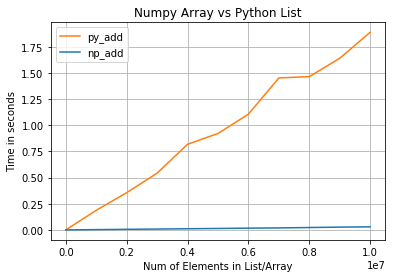
\includegraphics{images/vergleich_array_list.png}

Quelle: https://miro.medium.com/max/792/1*rQoLViAcg2Hj8AD1EmONAg.png

\hypertarget{vergleich-numpy-arrays-und-python-listen}{%
\subsubsection{Vergleich NumPy-Arrays und
Python-Listen}\label{vergleich-numpy-arrays-und-python-listen}}

Bei \emph{Python-Listen} werden die Anzahl der Elemente \textbf{nicht}
angegeben. Ebenso ist die Angabe des Datentyps nicht notwendig und
können demnach unterschiedlich sein. \emph{Python-Listen} sind Arrays
von Referenzen auf Daten. Diese Daten liegen im gesamten Arbeitsspeicher
(RAM) verstreut. Wird ein Element aufgerufen, wird auf die dazugehörige
Referenz geschaut und über diese auf das Objekt an einem Speicherort
zugegriffen. Dieser Vorgang führt zu Leistungseinbußen. Standardmäßig
sind \emph{Python-Listen} 1-Dimensional. Bei n-Dimensionale Listen
werden 1-Dimensionale Lists in einer weiteren 1-Dimensionale Liste
gespeichert.

Beim erzeugen von \emph{NumPy-Arrays} ist ein definierter Datentyp
notwendig. Falls kein Datentyp angegeben wird, verwenden
\emph{NumPy-Arrays} den Typ \emph{float}. Ebenso muss die Anzahl der
Elemente angegeben werden. Die Arrays werden zusammenhängend im RAM
gespeichert, was die Speichergröße im RAM deutlich verringert und für
einen einfacheren Zugriff auf die Daten sorgt.

\hypertarget{beispiel}{%
\subsubsection{Beispiel}\label{beispiel}}

Im Gegensatz zu \emph{Python-Listen} bieten \emph{NumPy-Arrays}
elementweise Operationen und damit gängige Vektor-Operationen. Die
folgenden Code-Beispiele verdeutlichen das. Dazu werden zwei
\emph{NumPy-Arrays} bzw. zwei \emph{Python-Listen} erstellt und
anschließend addiert. Zusätzlich wird eine der Arrays bzw. Listen mit
einem Skalar Multipliziert.

\textbf{Python-Listen:}

    \begin{tcolorbox}[breakable, size=fbox, boxrule=1pt, pad at break*=1mm,colback=cellbackground, colframe=cellborder]
\prompt{In}{incolor}{1}{\boxspacing}
\begin{Verbatim}[commandchars=\\\{\}]
\PY{n}{a} \PY{o}{=} \PY{p}{[}\PY{l+m+mi}{1}\PY{p}{,} \PY{l+m+mi}{2}\PY{p}{,} \PY{l+m+mi}{3}\PY{p}{]}
\PY{n}{b} \PY{o}{=} \PY{p}{[}\PY{l+m+mi}{4}\PY{p}{,} \PY{l+m+mi}{5}\PY{p}{,} \PY{l+m+mi}{6}\PY{p}{]}
\PY{n}{c} \PY{o}{=} \PY{l+m+mi}{3}

\PY{n+nb}{print}\PY{p}{(}\PY{l+s+s2}{\PYZdq{}}\PY{l+s+s2}{Addition:}\PY{l+s+s2}{\PYZdq{}}\PY{p}{,} \PY{p}{(}\PY{n}{a} \PY{o}{+} \PY{n}{b}\PY{p}{)}\PY{p}{)}
\PY{n+nb}{print}\PY{p}{(}\PY{l+s+s2}{\PYZdq{}}\PY{l+s+s2}{Multiplikation:}\PY{l+s+s2}{\PYZdq{}}\PY{p}{,} \PY{p}{(}\PY{n}{a} \PY{o}{*} \PY{n}{c}\PY{p}{)}\PY{p}{)}
\end{Verbatim}
\end{tcolorbox}

    \begin{Verbatim}[commandchars=\\\{\}]
Addition: [1, 2, 3, 4, 5, 6]
Multiplikation: [1, 2, 3, 1, 2, 3, 1, 2, 3]
    \end{Verbatim}

    Die Addition von zwei \emph{Python-Listen} sorgt für einen gängigen
Append. Das heißt, die Liste \textbf{b} wird an die Liste \textbf{a}
angehangen. Die Multiplikation der Liste \textbf{a} mit einem Skalar
\textbf{c} von 3 sorgt einfach für eine dreifache Wiederholung der
Liste.

\textbf{NumPy-Arrays:}

    \begin{tcolorbox}[breakable, size=fbox, boxrule=1pt, pad at break*=1mm,colback=cellbackground, colframe=cellborder]
\prompt{In}{incolor}{2}{\boxspacing}
\begin{Verbatim}[commandchars=\\\{\}]
\PY{k+kn}{import} \PY{n+nn}{numpy} \PY{k}{as} \PY{n+nn}{np}

\PY{n}{a} \PY{o}{=} \PY{n}{np}\PY{o}{.}\PY{n}{array}\PY{p}{(}\PY{p}{[}\PY{l+m+mi}{1}\PY{p}{,} \PY{l+m+mi}{2}\PY{p}{,} \PY{l+m+mi}{3}\PY{p}{]}\PY{p}{)}
\PY{n}{b} \PY{o}{=} \PY{n}{np}\PY{o}{.}\PY{n}{array}\PY{p}{(}\PY{p}{[}\PY{l+m+mi}{4}\PY{p}{,} \PY{l+m+mi}{5}\PY{p}{,} \PY{l+m+mi}{6}\PY{p}{]}\PY{p}{)}
\PY{n}{c} \PY{o}{=} \PY{l+m+mi}{3}

\PY{n+nb}{print}\PY{p}{(}\PY{l+s+s2}{\PYZdq{}}\PY{l+s+s2}{Addition:}\PY{l+s+s2}{\PYZdq{}}\PY{p}{,} \PY{p}{(}\PY{n}{a} \PY{o}{+} \PY{n}{b}\PY{p}{)}\PY{p}{)}
\PY{n+nb}{print}\PY{p}{(}\PY{l+s+s2}{\PYZdq{}}\PY{l+s+s2}{Multiplikation:}\PY{l+s+s2}{\PYZdq{}}\PY{p}{,} \PY{p}{(}\PY{n}{a} \PY{o}{*} \PY{n}{c}\PY{p}{)}\PY{p}{)}
\end{Verbatim}
\end{tcolorbox}

    \begin{Verbatim}[commandchars=\\\{\}]
Addition: [5 7 9]
Multiplikation: [3 6 9]
    \end{Verbatim}

    Werden statt \emph{Python-Listen} für die gleichen Operationen
\emph{NumPy-Arrays} verwendet, werden statt Appends gängige
mathematische Vektorberechnungen durchgeführt. So werden die Arrays
\textbf{a} und \textbf{b} elementweise addiert und das Skalar \textbf{c}
zu allen Elementen des Arrays \textbf{a} multipliziert.

Vektor- und Matrix-Berechnungen sind in der Digitalen Signalverarbeitung
sehr wichtig. Die Erweiterung von \emph{Python} durch
\emph{NumPy-Arrays} ist daher notwendig und bringt \emph{Python} so auf
das gleiche Level wie \emph{Matlab/Ocatve}.

    \hypertarget{scipy}{%
\subsection{SciPy}\label{scipy}}

\href{https://www.scipy.org/}{SciPy} ist eine Open-Source Bibliothek und
baut stark auf NumPy auf. Dadurch übernimmt es sämtliche im vorherigen
Kapitel genannten Geschwindigkeitsvorteile. Die Bibliothek erweitert
\emph{Python} um sehr viele Funktionen, welche für wissenschaftliches
und technisches Rechnen benötigt werden. Als Beispiel seien die
Funktionen für die
\href{https://scipy.github.io/devdocs/generated/scipy.signal.correlate.html}{Kreuzkorrelation}
und die
\href{https://scipy.github.io/devdocs/generated/scipy.fftpack.fft.html}{Fast
Fourier Transformation} genannt, welche auch in unserem Beispielprogramm
Anwendung finden.

Auf weitere Funktionen einzugehen würde den Rahmen dieses Dokuments
sprengen. Eine gute und strukturierte
\href{https://scipy.github.io/devdocs/}{Dokumentation} zu den
Funktionen, die \emph{SciPy} bietet, ist online zu finden.

\hypertarget{matplotlib}{%
\subsection{Matplotlib}\label{matplotlib}}

\href{https://matplotlib.org/}{Matplotlib} ist eine Bibliothek zum
Darstellen von einfachen Grafen und bis hin zu komplexen
3D-Darstellungen. So können Signale während der Verarbeitung zur
besseren Verständlichkeit grafisch dargestellt werden. Die Funktionen
sind dabei sehr ähnlich aufgebaut wie bei \emph{Matlab / Octave} und
bieten so eine einfache Übersetzung in die jeweils andere
Programmiersprache.

\hypertarget{beispielplot-octave}{%
\subsubsection{Beispielplot Octave}\label{beispielplot-octave}}

\begin{figure}
\centering
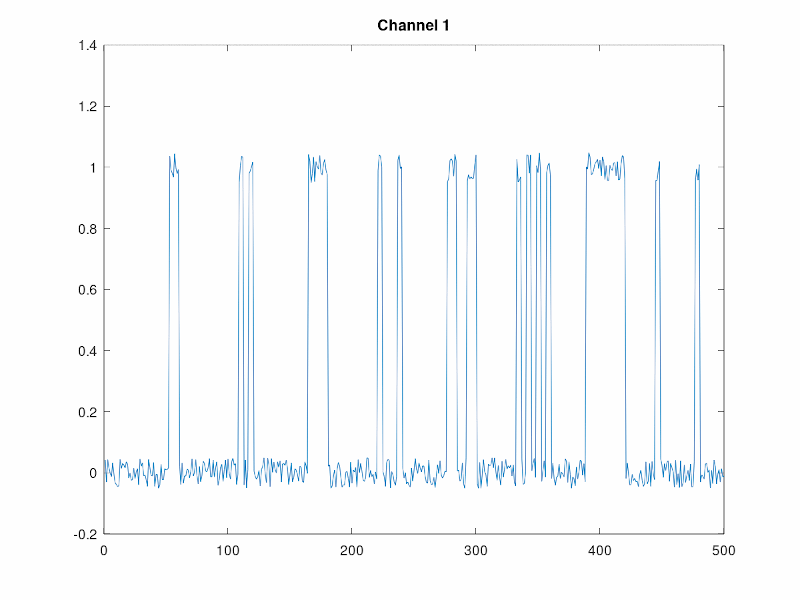
\includegraphics{images/plot_octave.png}
\caption{plot\_octave}
\end{figure}

\hypertarget{beispielplot-matplotlib}{%
\subsubsection{Beispielplot Matplotlib}\label{beispielplot-matplotlib}}

\begin{figure}
\centering
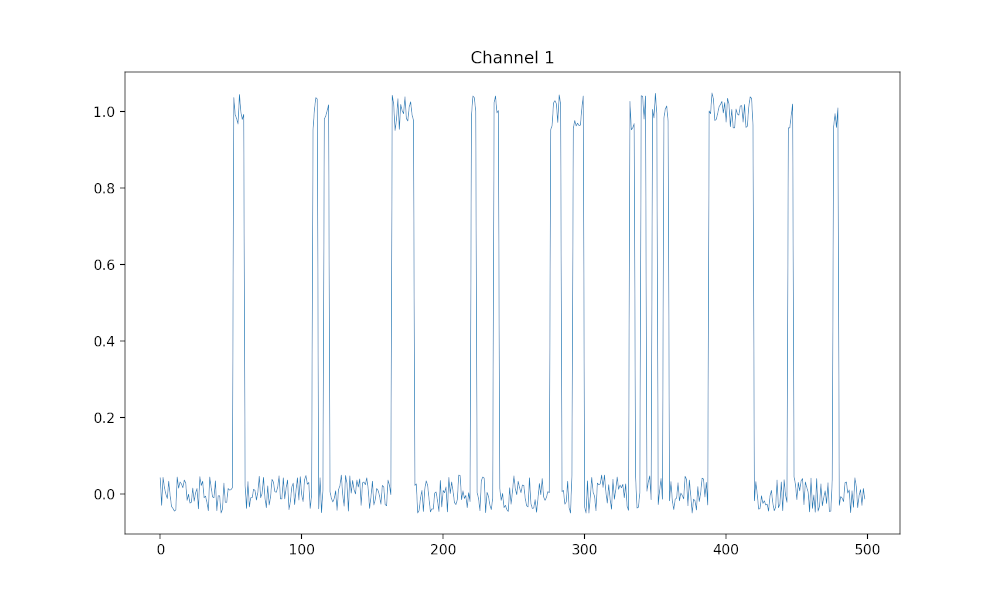
\includegraphics{images/plot_python.png}
\caption{plot\_python}
\end{figure}

\hypertarget{beispiel-3d-plot}{%
\subsubsection{Beispiel 3D-Plot}\label{beispiel-3d-plot}}

    \begin{tcolorbox}[breakable, size=fbox, boxrule=1pt, pad at break*=1mm,colback=cellbackground, colframe=cellborder]
\prompt{In}{incolor}{3}{\boxspacing}
\begin{Verbatim}[commandchars=\\\{\}]
\PY{k+kn}{import} \PY{n+nn}{matplotlib}\PY{n+nn}{.}\PY{n+nn}{pyplot} \PY{k}{as} \PY{n+nn}{plt}
\PY{k+kn}{from} \PY{n+nn}{matplotlib} \PY{k+kn}{import} \PY{n}{cm}
\PY{k+kn}{from} \PY{n+nn}{matplotlib}\PY{n+nn}{.}\PY{n+nn}{ticker} \PY{k+kn}{import} \PY{n}{LinearLocator}\PY{p}{,} \PY{n}{FormatStrFormatter}
\PY{k+kn}{import} \PY{n+nn}{numpy} \PY{k}{as} \PY{n+nn}{np}

\PY{n}{fig} \PY{o}{=} \PY{n}{plt}\PY{o}{.}\PY{n}{figure}\PY{p}{(}\PY{n}{dpi}\PY{o}{=}\PY{l+m+mi}{120}\PY{p}{)}
\PY{n}{ax} \PY{o}{=} \PY{n}{fig}\PY{o}{.}\PY{n}{gca}\PY{p}{(}\PY{n}{projection}\PY{o}{=}\PY{l+s+s1}{\PYZsq{}}\PY{l+s+s1}{3d}\PY{l+s+s1}{\PYZsq{}}\PY{p}{)}

\PY{c+c1}{\PYZsh{} Make data.}
\PY{n}{X} \PY{o}{=} \PY{n}{np}\PY{o}{.}\PY{n}{arange}\PY{p}{(}\PY{o}{\PYZhy{}}\PY{l+m+mi}{5}\PY{p}{,} \PY{l+m+mi}{5}\PY{p}{,} \PY{l+m+mf}{0.25}\PY{p}{)}
\PY{n}{Y} \PY{o}{=} \PY{n}{np}\PY{o}{.}\PY{n}{arange}\PY{p}{(}\PY{o}{\PYZhy{}}\PY{l+m+mi}{5}\PY{p}{,} \PY{l+m+mi}{5}\PY{p}{,} \PY{l+m+mf}{0.25}\PY{p}{)}
\PY{n}{X}\PY{p}{,} \PY{n}{Y} \PY{o}{=} \PY{n}{np}\PY{o}{.}\PY{n}{meshgrid}\PY{p}{(}\PY{n}{X}\PY{p}{,} \PY{n}{Y}\PY{p}{)}
\PY{n}{R} \PY{o}{=} \PY{n}{np}\PY{o}{.}\PY{n}{sqrt}\PY{p}{(}\PY{n}{X}\PY{o}{*}\PY{o}{*}\PY{l+m+mi}{2} \PY{o}{+} \PY{n}{Y}\PY{o}{*}\PY{o}{*}\PY{l+m+mi}{2}\PY{p}{)}
\PY{n}{Z} \PY{o}{=} \PY{n}{np}\PY{o}{.}\PY{n}{sin}\PY{p}{(}\PY{n}{R}\PY{p}{)}

\PY{c+c1}{\PYZsh{} Plot the surface.}
\PY{n}{surf} \PY{o}{=} \PY{n}{ax}\PY{o}{.}\PY{n}{plot\PYZus{}surface}\PY{p}{(}\PY{n}{X}\PY{p}{,} \PY{n}{Y}\PY{p}{,} \PY{n}{Z}\PY{p}{,} \PY{n}{cmap}\PY{o}{=}\PY{n}{cm}\PY{o}{.}\PY{n}{coolwarm}\PY{p}{,}
                       \PY{n}{linewidth}\PY{o}{=}\PY{l+m+mi}{0}\PY{p}{,} \PY{n}{antialiased}\PY{o}{=}\PY{k+kc}{False}\PY{p}{)}

\PY{c+c1}{\PYZsh{} Customize the z axis.}
\PY{n}{ax}\PY{o}{.}\PY{n}{set\PYZus{}zlim}\PY{p}{(}\PY{o}{\PYZhy{}}\PY{l+m+mf}{1.01}\PY{p}{,} \PY{l+m+mf}{1.01}\PY{p}{)}
\PY{n}{ax}\PY{o}{.}\PY{n}{zaxis}\PY{o}{.}\PY{n}{set\PYZus{}major\PYZus{}locator}\PY{p}{(}\PY{n}{LinearLocator}\PY{p}{(}\PY{l+m+mi}{10}\PY{p}{)}\PY{p}{)}
\PY{n}{ax}\PY{o}{.}\PY{n}{zaxis}\PY{o}{.}\PY{n}{set\PYZus{}major\PYZus{}formatter}\PY{p}{(}\PY{n}{FormatStrFormatter}\PY{p}{(}\PY{l+s+s1}{\PYZsq{}}\PY{l+s+si}{\PYZpc{}.02f}\PY{l+s+s1}{\PYZsq{}}\PY{p}{)}\PY{p}{)}

\PY{c+c1}{\PYZsh{} Add a color bar which maps values to colors.}
\PY{n}{fig}\PY{o}{.}\PY{n}{colorbar}\PY{p}{(}\PY{n}{surf}\PY{p}{,} \PY{n}{shrink}\PY{o}{=}\PY{l+m+mf}{0.5}\PY{p}{,} \PY{n}{aspect}\PY{o}{=}\PY{l+m+mi}{5}\PY{p}{)}

\PY{n}{plt}\PY{o}{.}\PY{n}{show}\PY{p}{(}\PY{p}{)}
\end{Verbatim}
\end{tcolorbox}

    \begin{center}
    \adjustimage{max size={0.9\linewidth}{0.9\paperheight}}{images/output_8_0.png}
    \end{center}
    { \hspace*{\fill} \\}
    
    Quelle: https://matplotlib.org/gallery/mplot3d/surface3d.html

    \hypertarget{code-vergleich}{%
\section{Code Vergleich}\label{code-vergleich}}

\hypertarget{entwicklung}{%
\subsection{Entwicklung}\label{entwicklung}}

Die Entwicklung eines Programms in \emph{Python}, das für die digitale
Signalverarbeitung verwendet wurde, umfasste eine Reihe von Schritten.
Zuerst wurde ein Programm in \emph{C} entwickelt, welches die Waveforms
erzeugte, die wir zur Simulation in unseren Programmen verarbeiteten.
Anschließend wurde in \emph{Octave} ein Skript entwickelt, das eine
Reihe von Basisoperationen in der digitalen Signalverarbeitung
durchführte. Dieses Skript wurde als Vorlage für den \emph{Python}-Code
und den \emph{C}-Code verwendet. Letzterer wurde nur zum
Geschwindigkeitsvergleich entwickelt und steht in dieser Ausarbeitung
nicht im Vordergrund. Bei der Entwicklung des \emph{Python}-Codes wurde
versucht den Code von \emph{Octave} 1:1 zu übernehmen. Sämtlicher für
diese Ausarbeitung geschriebener Code ist im Ordner ``code'' der
Ausarbeitung zu finden.

\hypertarget{beispielcode}{%
\subsection{Beispielcode}\label{beispielcode}}

Nachfolgend ist eine Reihe von Beispielen aus unserem
\emph{Python}-Codes und Vergleichcode aus dem \emph{Octave}-Basisskript
zu finden.

\hypertarget{vorbereitungen}{%
\subsubsection{Vorbereitungen}\label{vorbereitungen}}

Um die benötigten Operationen zu implementieren, wurden Funktionen aus
den Bibliotheken \emph{NumPy}, \emph{SciPy} und \emph{Matplotlib}
verwendet. Zusätzlich wurden die Waveforms, die zur Simulation dienen,
eingelesen. Da die Datenerfassung in der Praxis anders abläuft, wird an
dieser Stelle auf einen Vergleich mit dem \emph{Octave}-Code verzichtet.

    \begin{tcolorbox}[breakable, size=fbox, boxrule=1pt, pad at break*=1mm,colback=cellbackground, colframe=cellborder]
\prompt{In}{incolor}{4}{\boxspacing}
\begin{Verbatim}[commandchars=\\\{\}]
\PY{k+kn}{import} \PY{n+nn}{matplotlib}\PY{n+nn}{.}\PY{n+nn}{pyplot} \PY{k}{as} \PY{n+nn}{plt}
\PY{k+kn}{import} \PY{n+nn}{numpy} \PY{k}{as} \PY{n+nn}{np}
\PY{k+kn}{import} \PY{n+nn}{scipy}\PY{n+nn}{.}\PY{n+nn}{fftpack}
\PY{k+kn}{import} \PY{n+nn}{scipy}\PY{n+nn}{.}\PY{n+nn}{signal}

\PY{n}{ch1\PYZus{}foldername} \PY{o}{=} \PY{l+s+s2}{\PYZdq{}}\PY{l+s+s2}{ch1/}\PY{l+s+s2}{\PYZdq{}}
\PY{n}{ch2\PYZus{}foldername} \PY{o}{=} \PY{l+s+s2}{\PYZdq{}}\PY{l+s+s2}{ch2/}\PY{l+s+s2}{\PYZdq{}}
\PY{n}{ch3\PYZus{}foldername} \PY{o}{=} \PY{l+s+s2}{\PYZdq{}}\PY{l+s+s2}{ch3/}\PY{l+s+s2}{\PYZdq{}}
\PY{n}{wflen} \PY{o}{=} \PY{l+m+mi}{20000}
\PY{n}{avg\PYZus{}num} \PY{o}{=} \PY{l+m+mi}{16}                        \PY{c+c1}{\PYZsh{} max 128}

\PY{c+c1}{\PYZsh{}\PYZsh{}\PYZsh{} read waveform files into matrices \PYZsh{}\PYZsh{}\PYZsh{}\PYZsh{}\PYZsh{}\PYZsh{}\PYZsh{}\PYZsh{}\PYZsh{}\PYZsh{}\PYZsh{}\PYZsh{}\PYZsh{}\PYZsh{}\PYZsh{}\PYZsh{}\PYZsh{}\PYZsh{}\PYZsh{}\PYZsh{}\PYZsh{}\PYZsh{}\PYZsh{}\PYZsh{}\PYZsh{}\PYZsh{}\PYZsh{}\PYZsh{}\PYZsh{}\PYZsh{}\PYZsh{}\PYZsh{}\PYZsh{}\PYZsh{}\PYZsh{}\PYZsh{}\PYZsh{}\PYZsh{}\PYZsh{}\PYZsh{}\PYZsh{}\PYZsh{}}
\PY{n+nb}{print}\PY{p}{(}\PY{l+s+s2}{\PYZdq{}}\PY{l+s+s2}{read waveforms ...}\PY{l+s+s2}{\PYZdq{}}\PY{p}{,} \PY{n}{end}\PY{o}{=}\PY{l+s+s1}{\PYZsq{}}\PY{l+s+s1}{\PYZsq{}}\PY{p}{,} \PY{n}{flush}\PY{o}{=}\PY{k+kc}{True}\PY{p}{)}

\PY{n}{ch1\PYZus{}waveforms} \PY{o}{=} \PY{n}{np}\PY{o}{.}\PY{n}{empty}\PY{p}{(}\PY{p}{[}\PY{n}{avg\PYZus{}num}\PY{p}{,} \PY{n}{wflen}\PY{p}{]}\PY{p}{)}
\PY{n}{ch2\PYZus{}waveforms} \PY{o}{=} \PY{n}{np}\PY{o}{.}\PY{n}{empty}\PY{p}{(}\PY{p}{[}\PY{n}{avg\PYZus{}num}\PY{p}{,} \PY{n}{wflen}\PY{p}{]}\PY{p}{)}
\PY{n}{ch3\PYZus{}waveforms} \PY{o}{=} \PY{n}{np}\PY{o}{.}\PY{n}{empty}\PY{p}{(}\PY{p}{[}\PY{n}{avg\PYZus{}num}\PY{p}{,} \PY{n}{wflen}\PY{p}{]}\PY{p}{)}

\PY{k}{for} \PY{n}{i} \PY{o+ow}{in} \PY{n+nb}{range}\PY{p}{(}\PY{n}{avg\PYZus{}num}\PY{p}{)}\PY{p}{:}
    \PY{n}{filename} \PY{o}{=} \PY{l+s+s2}{\PYZdq{}}\PY{l+s+s2}{wf}\PY{l+s+s2}{\PYZdq{}} \PY{o}{+} \PY{n+nb}{str}\PY{p}{(}\PY{n}{i}\PY{o}{+}\PY{l+m+mi}{1}\PY{p}{)} \PY{o}{+} \PY{l+s+s2}{\PYZdq{}}\PY{l+s+s2}{.csv}\PY{l+s+s2}{\PYZdq{}}
    \PY{n}{ch1\PYZus{}waveforms}\PY{p}{[}\PY{n}{i}\PY{p}{]} \PY{o}{=} \PY{n}{np}\PY{o}{.}\PY{n}{genfromtxt}\PY{p}{(}\PY{n}{ch1\PYZus{}foldername} \PY{o}{+} \PY{n}{filename}\PY{p}{,} \PY{n}{delimiter}\PY{o}{=} \PY{l+s+s1}{\PYZsq{}}\PY{l+s+s1}{,}\PY{l+s+s1}{\PYZsq{}}\PY{p}{)}
    \PY{n}{ch2\PYZus{}waveforms}\PY{p}{[}\PY{n}{i}\PY{p}{]} \PY{o}{=} \PY{n}{np}\PY{o}{.}\PY{n}{genfromtxt}\PY{p}{(}\PY{n}{ch2\PYZus{}foldername} \PY{o}{+} \PY{n}{filename}\PY{p}{,} \PY{n}{delimiter}\PY{o}{=} \PY{l+s+s1}{\PYZsq{}}\PY{l+s+s1}{,}\PY{l+s+s1}{\PYZsq{}}\PY{p}{)}
    \PY{n}{ch3\PYZus{}waveforms}\PY{p}{[}\PY{n}{i}\PY{p}{]} \PY{o}{=} \PY{n}{np}\PY{o}{.}\PY{n}{genfromtxt}\PY{p}{(}\PY{n}{ch3\PYZus{}foldername} \PY{o}{+} \PY{n}{filename}\PY{p}{,} \PY{n}{delimiter}\PY{o}{=} \PY{l+s+s1}{\PYZsq{}}\PY{l+s+s1}{,}\PY{l+s+s1}{\PYZsq{}}\PY{p}{)}

\PY{n+nb}{print}\PY{p}{(}\PY{l+s+s2}{\PYZdq{}}\PY{l+s+s2}{done!}\PY{l+s+s2}{\PYZdq{}}\PY{p}{)}
\end{Verbatim}
\end{tcolorbox}

    \begin{Verbatim}[commandchars=\\\{\}]
read waveforms {\ldots}done!
    \end{Verbatim}

    \hypertarget{averaging}{%
\subsubsection{Averaging}\label{averaging}}

Als nächstes erstellten wir eine mit Nullen initialisierte Arrays für
die Mittelwertbildung der Waveforms. Dazu wurden die einzelnen Elemente
der Waveforms aufsummiert und durch die Anzahl der Aufsummierung
normiert. Dieses Verfahren dient zur Rauschminderung der Signale. Gut zu
sehen ist die Ähnlichkeit zwischen \emph{Python} und \emph{Octave}. Die
größten Unterschiede stellen die Syntax der For-Schleife und die
Indizierung der Einzelnen Elemente dar. \emph{Python} arbeitet wie
gängige Hochsprachen von 0 bis N-1, während \emph{Octave} wie in der
Elektrotechnik oft angewandt von 1 bis N zählt. Da \emph{Octave}
Matrixorientiert arbeitet und ein Vektoren einzeilige Matrizen
darstellen, müssen beim erstellen der Vektoren beide Dimensionen
angegeben werden. Dieser Schritt kann bei der Umsetzung in \emph{Python}
gespart werden.

    \hypertarget{python}{%
\paragraph{Python}\label{python}}

    \begin{tcolorbox}[breakable, size=fbox, boxrule=1pt, pad at break*=1mm,colback=cellbackground, colframe=cellborder]
\prompt{In}{incolor}{5}{\boxspacing}
\begin{Verbatim}[commandchars=\\\{\}]
\PY{n}{ch1\PYZus{}waveform\PYZus{}avg} \PY{o}{=} \PY{n}{np}\PY{o}{.}\PY{n}{zeros}\PY{p}{(}\PY{n}{wflen}\PY{p}{)}
\PY{n}{ch2\PYZus{}waveform\PYZus{}avg} \PY{o}{=} \PY{n}{np}\PY{o}{.}\PY{n}{zeros}\PY{p}{(}\PY{n}{wflen}\PY{p}{)}
\PY{n}{ch3\PYZus{}waveform\PYZus{}avg} \PY{o}{=} \PY{n}{np}\PY{o}{.}\PY{n}{zeros}\PY{p}{(}\PY{n}{wflen}\PY{p}{)}

\PY{k}{for} \PY{n}{i} \PY{o+ow}{in} \PY{n+nb}{range}\PY{p}{(}\PY{n}{avg\PYZus{}num}\PY{p}{)}\PY{p}{:}
    \PY{n}{ch1\PYZus{}waveform\PYZus{}avg} \PY{o}{+}\PY{o}{=} \PY{n}{ch1\PYZus{}waveforms}\PY{p}{[}\PY{n}{i}\PY{p}{]}
    \PY{n}{ch2\PYZus{}waveform\PYZus{}avg} \PY{o}{+}\PY{o}{=} \PY{n}{ch2\PYZus{}waveforms}\PY{p}{[}\PY{n}{i}\PY{p}{]}
    \PY{n}{ch3\PYZus{}waveform\PYZus{}avg} \PY{o}{+}\PY{o}{=} \PY{n}{ch3\PYZus{}waveforms}\PY{p}{[}\PY{n}{i}\PY{p}{]}

\PY{n}{ch1\PYZus{}waveform\PYZus{}avg} \PY{o}{/}\PY{o}{=} \PY{n}{avg\PYZus{}num}
\PY{n}{ch2\PYZus{}waveform\PYZus{}avg} \PY{o}{/}\PY{o}{=} \PY{n}{avg\PYZus{}num}
\PY{n}{ch3\PYZus{}waveform\PYZus{}avg} \PY{o}{/}\PY{o}{=} \PY{n}{avg\PYZus{}num}
\end{Verbatim}
\end{tcolorbox}

    \hypertarget{octave}{%
\paragraph{Octave}\label{octave}}

    \begin{tcolorbox}[breakable, size=fbox, boxrule=1pt, pad at break*=1mm,colback=cellbackground, colframe=cellborder]
\prompt{In}{incolor}{ }{\boxspacing}
\begin{Verbatim}[commandchars=\\\{\}]
\PY{n}{ch1\PYZus{}waveform\PYZus{}avg} \PY{o}{=} \PY{n}{zeros}\PY{p}{(}\PY{l+m+mi}{1}\PY{p}{,} \PY{n}{wflen}\PY{p}{)}\PY{p}{;}
\PY{n}{ch2\PYZus{}waveform\PYZus{}avg} \PY{o}{=} \PY{n}{zeros}\PY{p}{(}\PY{l+m+mi}{1}\PY{p}{,} \PY{n}{wflen}\PY{p}{)}\PY{p}{;}
\PY{n}{ch3\PYZus{}waveform\PYZus{}avg} \PY{o}{=} \PY{n}{zeros}\PY{p}{(}\PY{l+m+mi}{1}\PY{p}{,} \PY{n}{wflen}\PY{p}{)}\PY{p}{;}

\PY{k}{for} \PY{n}{i} \PY{o}{=} \PY{l+m+mi}{1}\PY{p}{:}\PY{n}{avg\PYZus{}num}
    \PY{n}{ch1\PYZus{}waveform\PYZus{}avg} \PY{o}{+}\PY{o}{=} \PY{n}{ch1\PYZus{}waveforms}\PY{p}{(}\PY{n}{i}\PY{p}{,} \PY{p}{:}\PY{p}{)}\PY{p}{;}
    \PY{n}{ch2\PYZus{}waveform\PYZus{}avg} \PY{o}{+}\PY{o}{=} \PY{n}{ch2\PYZus{}waveforms}\PY{p}{(}\PY{n}{i}\PY{p}{,} \PY{p}{:}\PY{p}{)}\PY{p}{;}
    \PY{n}{ch3\PYZus{}waveform\PYZus{}avg} \PY{o}{+}\PY{o}{=} \PY{n}{ch3\PYZus{}waveforms}\PY{p}{(}\PY{n}{i}\PY{p}{,} \PY{p}{:}\PY{p}{)}\PY{p}{;}
\PY{n}{endfor}

\PY{n}{ch1\PYZus{}waveform\PYZus{}avg} \PY{o}{/}\PY{o}{=} \PY{n}{avg\PYZus{}num}\PY{p}{;}
\PY{n}{ch2\PYZus{}waveform\PYZus{}avg} \PY{o}{/}\PY{o}{=} \PY{n}{avg\PYZus{}num}\PY{p}{;}
\PY{n}{ch3\PYZus{}waveform\PYZus{}avg} \PY{o}{/}\PY{o}{=} \PY{n}{avg\PYZus{}num}\PY{p}{;}
\end{Verbatim}
\end{tcolorbox}

    \hypertarget{upsampling}{%
\subsubsection{Upsampling}\label{upsampling}}

Das Upsampling wurde mit der Fast Fourier Transformation (fft) und der
Inversen Fast Fourier Transformation (ifft) aus der Bibliothek
\emph{SciPy} durchgeführt. Für das Einfügen der für das Upsampling
benötigten Nullen wird in \emph{Python} die Funktion
\emph{concatenate()} der Bibliothek \emph{NumPy} benötigt. In
\emph{Octave} sind für den Umgang mit Matrizen Operatoren vorhanden, was
sich in größeren Skripten als deutlich praktischer erweist. Auch hier
müssen wieder die Indizes beider Programmiersprachen beachtet werden.

    \hypertarget{python}{%
\paragraph{Python}\label{python}}

    \begin{tcolorbox}[breakable, size=fbox, boxrule=1pt, pad at break*=1mm,colback=cellbackground, colframe=cellborder]
\prompt{In}{incolor}{6}{\boxspacing}
\begin{Verbatim}[commandchars=\\\{\}]
\PY{n}{ch1\PYZus{}S} \PY{o}{=} \PY{n}{scipy}\PY{o}{.}\PY{n}{fftpack}\PY{o}{.}\PY{n}{fft}\PY{p}{(}\PY{n}{ch1\PYZus{}waveform\PYZus{}avg}\PY{p}{)}
\PY{n}{ch2\PYZus{}S} \PY{o}{=} \PY{n}{scipy}\PY{o}{.}\PY{n}{fftpack}\PY{o}{.}\PY{n}{fft}\PY{p}{(}\PY{n}{ch2\PYZus{}waveform\PYZus{}avg}\PY{p}{)}
\PY{n}{ch3\PYZus{}S} \PY{o}{=} \PY{n}{scipy}\PY{o}{.}\PY{n}{fftpack}\PY{o}{.}\PY{n}{fft}\PY{p}{(}\PY{n}{ch3\PYZus{}waveform\PYZus{}avg}\PY{p}{)}

\PY{n}{ch1\PYZus{}S\PYZus{}up} \PY{o}{=} \PY{n}{np}\PY{o}{.}\PY{n}{concatenate}\PY{p}{(}\PY{p}{(}\PY{n}{ch1\PYZus{}S}\PY{p}{[}\PY{l+m+mi}{0}\PY{p}{:}\PY{n+nb}{int}\PY{p}{(}\PY{n}{wflen}\PY{o}{/}\PY{l+m+mi}{2}\PY{p}{)}\PY{p}{]}\PY{p}{,} \PY{n}{np}\PY{o}{.}\PY{n}{zeros}\PY{p}{(}\PY{n}{wflen}\PY{p}{)}\PY{p}{,} \PY{n}{ch1\PYZus{}S}\PY{p}{[}\PY{n+nb}{int}\PY{p}{(}\PY{n}{wflen}\PY{o}{/}\PY{l+m+mi}{2}\PY{p}{)}\PY{p}{:}\PY{n}{wflen}\PY{p}{]}\PY{p}{)}\PY{p}{)}
\PY{n}{ch2\PYZus{}S\PYZus{}up} \PY{o}{=} \PY{n}{np}\PY{o}{.}\PY{n}{concatenate}\PY{p}{(}\PY{p}{(}\PY{n}{ch2\PYZus{}S}\PY{p}{[}\PY{l+m+mi}{0}\PY{p}{:}\PY{n+nb}{int}\PY{p}{(}\PY{n}{wflen}\PY{o}{/}\PY{l+m+mi}{2}\PY{p}{)}\PY{p}{]}\PY{p}{,} \PY{n}{np}\PY{o}{.}\PY{n}{zeros}\PY{p}{(}\PY{n}{wflen}\PY{p}{)}\PY{p}{,} \PY{n}{ch2\PYZus{}S}\PY{p}{[}\PY{n+nb}{int}\PY{p}{(}\PY{n}{wflen}\PY{o}{/}\PY{l+m+mi}{2}\PY{p}{)}\PY{p}{:}\PY{n}{wflen}\PY{p}{]}\PY{p}{)}\PY{p}{)}
\PY{n}{ch3\PYZus{}S\PYZus{}up} \PY{o}{=} \PY{n}{np}\PY{o}{.}\PY{n}{concatenate}\PY{p}{(}\PY{p}{(}\PY{n}{ch3\PYZus{}S}\PY{p}{[}\PY{l+m+mi}{0}\PY{p}{:}\PY{n+nb}{int}\PY{p}{(}\PY{n}{wflen}\PY{o}{/}\PY{l+m+mi}{2}\PY{p}{)}\PY{p}{]}\PY{p}{,} \PY{n}{np}\PY{o}{.}\PY{n}{zeros}\PY{p}{(}\PY{n}{wflen}\PY{p}{)}\PY{p}{,} \PY{n}{ch3\PYZus{}S}\PY{p}{[}\PY{n+nb}{int}\PY{p}{(}\PY{n}{wflen}\PY{o}{/}\PY{l+m+mi}{2}\PY{p}{)}\PY{p}{:}\PY{n}{wflen}\PY{p}{]}\PY{p}{)}\PY{p}{)}

\PY{n}{ch1\PYZus{}waveform\PYZus{}upsamp} \PY{o}{=} \PY{n}{np}\PY{o}{.}\PY{n}{real}\PY{p}{(}\PY{n}{scipy}\PY{o}{.}\PY{n}{fftpack}\PY{o}{.}\PY{n}{ifft}\PY{p}{(}\PY{n}{ch1\PYZus{}S\PYZus{}up}\PY{p}{)}\PY{p}{)} \PY{o}{*} \PY{l+m+mi}{2}
\PY{n}{ch2\PYZus{}waveform\PYZus{}upsamp} \PY{o}{=} \PY{n}{np}\PY{o}{.}\PY{n}{real}\PY{p}{(}\PY{n}{scipy}\PY{o}{.}\PY{n}{fftpack}\PY{o}{.}\PY{n}{ifft}\PY{p}{(}\PY{n}{ch2\PYZus{}S\PYZus{}up}\PY{p}{)}\PY{p}{)} \PY{o}{*} \PY{l+m+mi}{2}
\PY{n}{ch3\PYZus{}waveform\PYZus{}upsamp} \PY{o}{=} \PY{n}{np}\PY{o}{.}\PY{n}{real}\PY{p}{(}\PY{n}{scipy}\PY{o}{.}\PY{n}{fftpack}\PY{o}{.}\PY{n}{ifft}\PY{p}{(}\PY{n}{ch3\PYZus{}S\PYZus{}up}\PY{p}{)}\PY{p}{)} \PY{o}{*} \PY{l+m+mi}{2}

\PY{n}{wflen} \PY{o}{*}\PY{o}{=} \PY{l+m+mi}{2}
\end{Verbatim}
\end{tcolorbox}

    \hypertarget{octave}{%
\paragraph{Octave}\label{octave}}

    \begin{tcolorbox}[breakable, size=fbox, boxrule=1pt, pad at break*=1mm,colback=cellbackground, colframe=cellborder]
\prompt{In}{incolor}{ }{\boxspacing}
\begin{Verbatim}[commandchars=\\\{\}]
\PY{n}{ch1\PYZus{}S} \PY{o}{=} \PY{n}{fft}\PY{p}{(}\PY{n}{ch1\PYZus{}waveform\PYZus{}avg}\PY{p}{)}\PY{p}{;}
\PY{n}{ch2\PYZus{}S} \PY{o}{=} \PY{n}{fft}\PY{p}{(}\PY{n}{ch2\PYZus{}waveform\PYZus{}avg}\PY{p}{)}\PY{p}{;}
\PY{n}{ch3\PYZus{}S} \PY{o}{=} \PY{n}{fft}\PY{p}{(}\PY{n}{ch3\PYZus{}waveform\PYZus{}avg}\PY{p}{)}\PY{p}{;}

\PY{n}{ch1\PYZus{}S\PYZus{}up} \PY{o}{=} \PY{p}{[}\PY{n}{ch1\PYZus{}S}\PY{p}{(}\PY{l+m+mi}{1}\PY{p}{:}\PY{n}{wflen}\PY{o}{/}\PY{l+m+mi}{2}\PY{p}{)}\PY{p}{,} \PY{n}{zeros}\PY{p}{(}\PY{l+m+mi}{1}\PY{p}{,} \PY{n}{wflen}\PY{p}{)}\PY{p}{,} \PY{n}{ch1\PYZus{}S}\PY{p}{(}\PY{n}{wflen}\PY{o}{/}\PY{l+m+mi}{2}\PY{o}{+}\PY{l+m+mi}{1}\PY{p}{:}\PY{n}{wflen}\PY{p}{)}\PY{p}{]}\PY{p}{;}
\PY{n}{ch2\PYZus{}S\PYZus{}up} \PY{o}{=} \PY{p}{[}\PY{n}{ch2\PYZus{}S}\PY{p}{(}\PY{l+m+mi}{1}\PY{p}{:}\PY{n}{wflen}\PY{o}{/}\PY{l+m+mi}{2}\PY{p}{)}\PY{p}{,} \PY{n}{zeros}\PY{p}{(}\PY{l+m+mi}{1}\PY{p}{,} \PY{n}{wflen}\PY{p}{)}\PY{p}{,} \PY{n}{ch2\PYZus{}S}\PY{p}{(}\PY{n}{wflen}\PY{o}{/}\PY{l+m+mi}{2}\PY{o}{+}\PY{l+m+mi}{1}\PY{p}{:}\PY{n}{wflen}\PY{p}{)}\PY{p}{]}\PY{p}{;}
\PY{n}{ch3\PYZus{}S\PYZus{}up} \PY{o}{=} \PY{p}{[}\PY{n}{ch3\PYZus{}S}\PY{p}{(}\PY{l+m+mi}{1}\PY{p}{:}\PY{n}{wflen}\PY{o}{/}\PY{l+m+mi}{2}\PY{p}{)}\PY{p}{,} \PY{n}{zeros}\PY{p}{(}\PY{l+m+mi}{1}\PY{p}{,} \PY{n}{wflen}\PY{p}{)}\PY{p}{,} \PY{n}{ch3\PYZus{}S}\PY{p}{(}\PY{n}{wflen}\PY{o}{/}\PY{l+m+mi}{2}\PY{o}{+}\PY{l+m+mi}{1}\PY{p}{:}\PY{n}{wflen}\PY{p}{)}\PY{p}{]}\PY{p}{;}

\PY{n}{ch1\PYZus{}waveform\PYZus{}upsamp} \PY{o}{=} \PY{n}{real}\PY{p}{(}\PY{n}{ifft}\PY{p}{(}\PY{n}{ch1\PYZus{}S\PYZus{}up}\PY{p}{)}\PY{p}{)} \PY{o}{*} \PY{l+m+mi}{2}\PY{p}{;}
\PY{n}{ch2\PYZus{}waveform\PYZus{}upsamp} \PY{o}{=} \PY{n}{real}\PY{p}{(}\PY{n}{ifft}\PY{p}{(}\PY{n}{ch2\PYZus{}S\PYZus{}up}\PY{p}{)}\PY{p}{)} \PY{o}{*} \PY{l+m+mi}{2}\PY{p}{;}
\PY{n}{ch3\PYZus{}waveform\PYZus{}upsamp} \PY{o}{=} \PY{n}{real}\PY{p}{(}\PY{n}{ifft}\PY{p}{(}\PY{n}{ch3\PYZus{}S\PYZus{}up}\PY{p}{)}\PY{p}{)} \PY{o}{*} \PY{l+m+mi}{2}\PY{p}{;}

\PY{n}{wflen} \PY{o}{*}\PY{o}{=} \PY{l+m+mi}{2}\PY{p}{;}
\end{Verbatim}
\end{tcolorbox}

    \hypertarget{laufluxe4ngenkorrektur-und-combining}{%
\subsubsection{Lauflängenkorrektur und
combining}\label{laufluxe4ngenkorrektur-und-combining}}

Schließlich wurde eine Lauflänge Korrektur und eine simples Combining
der Waveforms durchgeführt. Dabei musste besonders auf den Unterschied
der Indizes in \emph{Python} und \emph{Oktave} achten, um
sicherzustellen, dass die zu korrelierenden und zu kombinierten Elemente
die gleiche Länge hatten und die Vektoren an den richtigen Stellen
begannen und endeten.

    \hypertarget{python}{%
\paragraph{Python}\label{python}}

    \begin{tcolorbox}[breakable, size=fbox, boxrule=1pt, pad at break*=1mm,colback=cellbackground, colframe=cellborder]
\prompt{In}{incolor}{7}{\boxspacing}
\begin{Verbatim}[commandchars=\\\{\}]
\PY{n}{normVec} \PY{o}{=} \PY{n}{np}\PY{o}{.}\PY{n}{append}\PY{p}{(}\PY{n}{np}\PY{o}{.}\PY{n}{arange}\PY{p}{(}\PY{l+m+mi}{1}\PY{p}{,} \PY{n}{wflen}\PY{o}{+}\PY{l+m+mi}{1}\PY{p}{)}\PY{p}{,} \PY{n}{np}\PY{o}{.}\PY{n}{arange}\PY{p}{(}\PY{n}{wflen}\PY{o}{\PYZhy{}}\PY{l+m+mi}{1}\PY{p}{,} \PY{l+m+mi}{0}\PY{p}{,} \PY{o}{\PYZhy{}}\PY{l+m+mi}{1}\PY{p}{)}\PY{p}{)}

\PY{n}{corr2} \PY{o}{=} \PY{n}{scipy}\PY{o}{.}\PY{n}{signal}\PY{o}{.}\PY{n}{correlate}\PY{p}{(}\PY{n}{ch1\PYZus{}waveform\PYZus{}upsamp}\PY{p}{,} \PY{n}{ch2\PYZus{}waveform\PYZus{}upsamp}\PY{p}{)} \PY{o}{/} \PY{n}{normVec}
\PY{n}{corr3} \PY{o}{=} \PY{n}{scipy}\PY{o}{.}\PY{n}{signal}\PY{o}{.}\PY{n}{correlate}\PY{p}{(}\PY{n}{ch1\PYZus{}waveform\PYZus{}upsamp}\PY{p}{,} \PY{n}{ch3\PYZus{}waveform\PYZus{}upsamp}\PY{p}{)} \PY{o}{/} \PY{n}{normVec}

\PY{n}{trunc} \PY{o}{=} \PY{n+nb}{int}\PY{p}{(}\PY{n+nb}{len}\PY{p}{(}\PY{n}{corr2}\PY{p}{)}\PY{o}{/}\PY{l+m+mi}{100} \PY{o}{*} \PY{l+m+mi}{5}\PY{p}{)}\PY{p}{;}                    \PY{c+c1}{\PYZsh{} 5\PYZpc{} truncatination}
\PY{n}{idx2} \PY{o}{=} \PY{n}{np}\PY{o}{.}\PY{n}{argmax}\PY{p}{(}\PY{n}{corr2}\PY{p}{[}\PY{n}{trunc}\PY{p}{:}\PY{n+nb}{len}\PY{p}{(}\PY{n}{corr2}\PY{p}{)}\PY{o}{\PYZhy{}}\PY{n}{trunc}\PY{p}{]}\PY{p}{)}     \PY{c+c1}{\PYZsh{} don\PYZsq{}t use 5\PYZpc{} of waveform ends}
\PY{n}{idx3} \PY{o}{=} \PY{n}{np}\PY{o}{.}\PY{n}{argmax}\PY{p}{(}\PY{n}{corr3}\PY{p}{[}\PY{n}{trunc}\PY{p}{:}\PY{n+nb}{len}\PY{p}{(}\PY{n}{corr3}\PY{p}{)}\PY{o}{\PYZhy{}}\PY{n}{trunc}\PY{p}{]}\PY{p}{)}
\PY{n}{idx2} \PY{o}{+}\PY{o}{=} \PY{p}{(}\PY{n}{trunc} \PY{o}{+} \PY{l+m+mi}{1}\PY{p}{)}                                 \PY{c+c1}{\PYZsh{} addition of trunc, to get correct index}
\PY{n}{idx3} \PY{o}{+}\PY{o}{=} \PY{p}{(}\PY{n}{trunc} \PY{o}{+} \PY{l+m+mi}{1}\PY{p}{)}
\PY{n}{shift2} \PY{o}{=} \PY{n}{idx2} \PY{o}{\PYZhy{}} \PY{n}{wflen}
\PY{n}{shift3} \PY{o}{=} \PY{n}{idx3} \PY{o}{\PYZhy{}} \PY{n}{wflen}

\PY{n}{ch1\PYZus{}waveform\PYZus{}shifted} \PY{o}{=} \PY{n}{ch1\PYZus{}waveform\PYZus{}upsamp}\PY{p}{[}\PY{n}{shift3}\PY{p}{:}\PY{n}{wflen}\PY{p}{]}
\PY{n}{ch2\PYZus{}waveform\PYZus{}shifted} \PY{o}{=} \PY{n}{ch2\PYZus{}waveform\PYZus{}upsamp}\PY{p}{[}\PY{n}{shift2}\PY{p}{:}\PY{n}{wflen}\PY{o}{\PYZhy{}}\PY{n}{shift2}\PY{p}{]}
\PY{n}{ch3\PYZus{}waveform\PYZus{}shifted} \PY{o}{=} \PY{n}{ch3\PYZus{}waveform\PYZus{}upsamp}\PY{p}{[}\PY{l+m+mi}{0}\PY{p}{:}\PY{n}{wflen}\PY{o}{\PYZhy{}}\PY{n}{shift3}\PY{p}{]}

\PY{n}{comb} \PY{o}{=} \PY{n}{ch1\PYZus{}waveform\PYZus{}shifted} \PY{o}{+} \PY{n}{ch2\PYZus{}waveform\PYZus{}shifted} \PY{o}{+} \PY{n}{ch3\PYZus{}waveform\PYZus{}shifted}
\end{Verbatim}
\end{tcolorbox}

    \hypertarget{octave}{%
\paragraph{Octave}\label{octave}}

    \begin{tcolorbox}[breakable, size=fbox, boxrule=1pt, pad at break*=1mm,colback=cellbackground, colframe=cellborder]
\prompt{In}{incolor}{ }{\boxspacing}
\begin{Verbatim}[commandchars=\\\{\}]
\PY{n}{normVec} \PY{o}{=} \PY{p}{[}\PY{p}{(}\PY{l+m+mi}{1}\PY{p}{:}\PY{n}{wflen}\PY{p}{)}\PY{p}{,} \PY{n}{fliplr}\PY{p}{(}\PY{l+m+mi}{1}\PY{p}{:}\PY{n}{wflen}\PY{o}{\PYZhy{}}\PY{l+m+mi}{1}\PY{p}{)}\PY{p}{]}\PY{p}{;}

\PY{n}{corr2} \PY{o}{=} \PY{n}{xcorr}\PY{p}{(}\PY{n}{ch1\PYZus{}waveform\PYZus{}upsamp}\PY{p}{,} \PY{n}{ch2\PYZus{}waveform\PYZus{}upsamp}\PY{p}{)} \PY{o}{.}\PY{o}{/} \PY{n}{normVec}\PY{p}{;}
\PY{n}{corr3} \PY{o}{=} \PY{n}{xcorr}\PY{p}{(}\PY{n}{ch1\PYZus{}waveform\PYZus{}upsamp}\PY{p}{,} \PY{n}{ch3\PYZus{}waveform\PYZus{}upsamp}\PY{p}{)} \PY{o}{.}\PY{o}{/} \PY{n}{normVec}\PY{p}{;}

\PY{n}{trunc} \PY{o}{=} \PY{n}{ceil}\PY{p}{(}\PY{n}{length}\PY{p}{(}\PY{n}{corr2}\PY{p}{)} \PY{o}{/} \PY{l+m+mi}{100} \PY{o}{*} \PY{l+m+mi}{5}\PY{p}{)}\PY{p}{;}          \PY{c+c1}{\PYZsh{} 5\PYZpc{} truncatination}
\PY{p}{[}\PY{n}{val2}\PY{p}{,} \PY{n}{idx2}\PY{p}{]} \PY{o}{=} \PY{n+nb}{max}\PY{p}{(}\PY{n}{corr2}\PY{p}{(}\PY{n}{trunc}\PY{p}{:}\PY{n}{end}\PY{o}{\PYZhy{}}\PY{n}{trunc}\PY{p}{)}\PY{p}{)}\PY{p}{;}     \PY{c+c1}{\PYZsh{} don\PYZsq{}t use 5\PYZpc{} of waveform ends}
\PY{p}{[}\PY{n}{val3}\PY{p}{,} \PY{n}{idx3}\PY{p}{]} \PY{o}{=} \PY{n+nb}{max}\PY{p}{(}\PY{n}{corr3}\PY{p}{(}\PY{n}{trunc}\PY{p}{:}\PY{n}{end}\PY{o}{\PYZhy{}}\PY{n}{trunc}\PY{p}{)}\PY{p}{)}\PY{p}{;}
\PY{n}{idx2} \PY{o}{+}\PY{o}{=} \PY{p}{(}\PY{n}{trunc} \PY{o}{\PYZhy{}} \PY{l+m+mi}{1}\PY{p}{)}\PY{p}{;}                            \PY{c+c1}{\PYZsh{} addition of trunc, to get correct index}
\PY{n}{idx3} \PY{o}{+}\PY{o}{=} \PY{p}{(}\PY{n}{trunc} \PY{o}{\PYZhy{}} \PY{l+m+mi}{1}\PY{p}{)}\PY{p}{;}
\PY{n}{shift2} \PY{o}{=} \PY{n}{idx2} \PY{o}{\PYZhy{}} \PY{n}{wflen}\PY{p}{;}
\PY{n}{shift3} \PY{o}{=} \PY{n}{idx3} \PY{o}{\PYZhy{}} \PY{n}{wflen}\PY{p}{;}

\PY{n}{ch1\PYZus{}waveform\PYZus{}shifted} \PY{o}{=} \PY{n}{ch1\PYZus{}waveform\PYZus{}upsamp}\PY{p}{(}\PY{n}{shift3}\PY{o}{+}\PY{l+m+mi}{1}\PY{p}{:}\PY{n}{wflen}\PY{p}{)}\PY{p}{;}
\PY{n}{ch2\PYZus{}waveform\PYZus{}shifted} \PY{o}{=} \PY{n}{ch2\PYZus{}waveform\PYZus{}upsamp}\PY{p}{(}\PY{n}{shift2}\PY{o}{+}\PY{l+m+mi}{1}\PY{p}{:}\PY{n}{wflen}\PY{o}{\PYZhy{}}\PY{n}{shift2}\PY{p}{)}\PY{p}{;}
\PY{n}{ch3\PYZus{}waveform\PYZus{}shifted} \PY{o}{=} \PY{n}{ch3\PYZus{}waveform\PYZus{}upsamp}\PY{p}{(}\PY{l+m+mi}{1}\PY{p}{:}\PY{n}{wflen}\PY{o}{\PYZhy{}}\PY{n}{shift3}\PY{p}{)}\PY{p}{;}

\PY{n}{comb} \PY{o}{=} \PY{n}{ch1\PYZus{}waveform\PYZus{}shifted} \PY{o}{.}\PY{o}{+} \PY{n}{ch2\PYZus{}waveform\PYZus{}shifted} \PY{o}{.}\PY{o}{+} \PY{n}{ch3\PYZus{}waveform\PYZus{}shifted}\PY{p}{;}
\end{Verbatim}
\end{tcolorbox}

    \hypertarget{plot}{%
\subsubsection{Plot}\label{plot}}

Zur besseren Veranschaulichung können die Waveform grafisch dargestellt
werden. Auch diese Funktionalität ist bei \emph{Octave} standardmäßig
integriert. \emph{Python} muss durch die Bibliothek \emph{Matplotlib}
erweitert werden, um diese Plots zu bieten. Die grafische Darstellung
von Subplots gelingt \emph{Octave} etwas besser. Bei \emph{Python} wird
die zusätzliche Funktion \emph{tight\_layout} benötigt, da sonst die
Titel der Plots von den darunterliegenden Plots verdeckt werden.

    \hypertarget{python}{%
\paragraph{Python}\label{python}}

    \begin{tcolorbox}[breakable, size=fbox, boxrule=1pt, pad at break*=1mm,colback=cellbackground, colframe=cellborder]
\prompt{In}{incolor}{8}{\boxspacing}
\begin{Verbatim}[commandchars=\\\{\}]
\PY{n}{plt}\PY{o}{.}\PY{n}{figure}\PY{p}{(}\PY{l+m+mi}{1}\PY{p}{)}

\PY{n}{plt}\PY{o}{.}\PY{n}{subplot}\PY{p}{(}\PY{l+m+mi}{311}\PY{p}{)}
\PY{n}{plt}\PY{o}{.}\PY{n}{title}\PY{p}{(}\PY{l+s+s2}{\PYZdq{}}\PY{l+s+s2}{Channel 1}\PY{l+s+s2}{\PYZdq{}}\PY{p}{)}
\PY{n}{plt}\PY{o}{.}\PY{n}{tight\PYZus{}layout}\PY{p}{(}\PY{p}{)}
\PY{n}{plt}\PY{o}{.}\PY{n}{plot}\PY{p}{(}\PY{n}{ch1\PYZus{}waveforms}\PY{p}{[}\PY{l+m+mi}{0}\PY{p}{,} \PY{l+m+mi}{0}\PY{p}{:}\PY{l+m+mi}{499}\PY{p}{]}\PY{p}{)}

\PY{n}{plt}\PY{o}{.}\PY{n}{subplot}\PY{p}{(}\PY{l+m+mi}{312}\PY{p}{)}
\PY{n}{plt}\PY{o}{.}\PY{n}{title}\PY{p}{(}\PY{l+s+s2}{\PYZdq{}}\PY{l+s+s2}{Channel 1 averaged}\PY{l+s+s2}{\PYZdq{}}\PY{p}{)}
\PY{n}{plt}\PY{o}{.}\PY{n}{tight\PYZus{}layout}\PY{p}{(}\PY{p}{)}
\PY{n}{plt}\PY{o}{.}\PY{n}{plot}\PY{p}{(}\PY{n}{ch1\PYZus{}waveform\PYZus{}avg}\PY{p}{[}\PY{l+m+mi}{0}\PY{p}{:}\PY{l+m+mi}{499}\PY{p}{]}\PY{p}{)}

\PY{n}{plt}\PY{o}{.}\PY{n}{subplot}\PY{p}{(}\PY{l+m+mi}{313}\PY{p}{)}
\PY{n}{plt}\PY{o}{.}\PY{n}{title}\PY{p}{(}\PY{l+s+s2}{\PYZdq{}}\PY{l+s+s2}{Channel 1 upsampled}\PY{l+s+s2}{\PYZdq{}}\PY{p}{)}
\PY{n}{plt}\PY{o}{.}\PY{n}{tight\PYZus{}layout}\PY{p}{(}\PY{p}{)}
\PY{n}{plt}\PY{o}{.}\PY{n}{plot}\PY{p}{(}\PY{n}{ch1\PYZus{}waveform\PYZus{}upsamp}\PY{p}{[}\PY{l+m+mi}{0}\PY{p}{:}\PY{l+m+mi}{999}\PY{p}{]}\PY{p}{)}
\end{Verbatim}
\end{tcolorbox}

            \begin{tcolorbox}[breakable, size=fbox, boxrule=.5pt, pad at break*=1mm, opacityfill=0]
\prompt{Out}{outcolor}{8}{\boxspacing}
\begin{Verbatim}[commandchars=\\\{\}]
[<matplotlib.lines.Line2D at 0x2682682deb0>]
\end{Verbatim}
\end{tcolorbox}
        
    \begin{center}
    \adjustimage{max size={0.9\linewidth}{0.9\paperheight}}{images/output_29_1.png}
    \end{center}
    { \hspace*{\fill} \\}
    
    \hypertarget{octave}{%
\paragraph{Octave}\label{octave}}

    \begin{tcolorbox}[breakable, size=fbox, boxrule=1pt, pad at break*=1mm,colback=cellbackground, colframe=cellborder]
\prompt{In}{incolor}{ }{\boxspacing}
\begin{Verbatim}[commandchars=\\\{\}]
\PY{n}{figure}\PY{p}{(}\PY{l+m+mi}{1}\PY{p}{)}\PY{p}{;}

\PY{n}{subplot}\PY{p}{(}\PY{l+m+mi}{3}\PY{p}{,} \PY{l+m+mi}{1}\PY{p}{,} \PY{l+m+mi}{1}\PY{p}{)}\PY{p}{;}
\PY{n}{plot}\PY{p}{(}\PY{n}{ch1\PYZus{}waveforms}\PY{p}{(}\PY{l+m+mi}{1}\PY{p}{,} \PY{l+m+mi}{1}\PY{p}{:}\PY{l+m+mi}{500}\PY{p}{)}\PY{p}{)}\PY{p}{;}
\PY{n}{title}\PY{p}{(}\PY{l+s+s2}{\PYZdq{}}\PY{l+s+s2}{Channel 1}\PY{l+s+s2}{\PYZdq{}}\PY{p}{)}\PY{p}{;}

\PY{n}{subplot}\PY{p}{(}\PY{l+m+mi}{3}\PY{p}{,} \PY{l+m+mi}{1}\PY{p}{,} \PY{l+m+mi}{2}\PY{p}{)}\PY{p}{;}
\PY{n}{plot}\PY{p}{(}\PY{n}{ch1\PYZus{}waveform\PYZus{}avg}\PY{p}{(}\PY{l+m+mi}{1}\PY{p}{:}\PY{l+m+mi}{500}\PY{p}{)}\PY{p}{)}\PY{p}{;}
\PY{n}{title}\PY{p}{(}\PY{l+s+s2}{\PYZdq{}}\PY{l+s+s2}{Channel 1 averaged}\PY{l+s+s2}{\PYZdq{}}\PY{p}{)}\PY{p}{;}

\PY{n}{subplot}\PY{p}{(}\PY{l+m+mi}{3}\PY{p}{,} \PY{l+m+mi}{1}\PY{p}{,} \PY{l+m+mi}{3}\PY{p}{)}\PY{p}{;}
\PY{n}{plot}\PY{p}{(}\PY{n}{ch1\PYZus{}waveform\PYZus{}upsamp}\PY{p}{(}\PY{l+m+mi}{1}\PY{p}{:}\PY{l+m+mi}{1000}\PY{p}{)}\PY{p}{)}\PY{p}{;}
\PY{n}{title}\PY{p}{(}\PY{l+s+s2}{\PYZdq{}}\PY{l+s+s2}{Channel 1 upsampled}\PY{l+s+s2}{\PYZdq{}}\PY{p}{)}\PY{p}{;}
\end{Verbatim}
\end{tcolorbox}

    \hypertarget{gegenuxfcberstellung-von-python-und-octave}{%
\subsection{Gegenüberstellung von Python und
Octave}\label{gegenuxfcberstellung-von-python-und-octave}}

\hypertarget{vorteile-von-python}{%
\subsubsection{Vorteile von Python}\label{vorteile-von-python}}

Der Hauptvorteil von \emph{Python} gegenüber \emph{Octave} besteht
darin, dass es sich bei \emph{Python} um eine allgemeine Hochsprachen
handelt. Das bedeutet, dass \emph{Python} weitaus vielseitiger und
flexibler ist, als \emph{Octave}, und so zur Bewältigung von
verschiedenen Arten von Aufgaben eingesetzt werden kann. Es ist
einfacher und eleganter, eine einzige Sprache für alle in einem Projekt
benötigten Aufgaben zu verwenden. Ein weiterer wichtiger Vorteil von
\emph{Python} gegenüber \emph{Matlab} (aber nicht \emph{Octave}) ist,
dass es sich bei \emph{Python} um ein Open-Source-Projekt handelt. Die
Vorteile von Open-Source-Software gehen weit über den offensichtlichen
Vorteil hinaus, dass sie kostenlos ist. Zusätzlich profitiert
Open-Source-Software davon, dass sie eine größere, verteilte
Entwicklergemeinde hat und ihre weitere Entwicklung nicht vom
Fortbestand eines Unternehmens abhängig ist. Auch die Verwendung von
Open-Source-Software macht es für Dritte einfacher, den Code und die
Ergebnisse jeder Arbeit, die man veröffentlicht, zu verwenden und zu
überprüfen, da sie einfach die dafür notwendige Software herunterladen
können und nicht für proprietäre Software bezahlen müssen, wenn sie die
eigene Arbeit nutzen wollen.

\hypertarget{vorteile-von-octave}{%
\subsubsection{Vorteile von Octave}\label{vorteile-von-octave}}

Der Vorteil von \emph{Octave/Matlab} besteht darin, dass sie speziell
für diese Art von Aufgaben entwickelt wurden. Dadurch sind alle
notwendigen Funktionen bereits enthalten und sehr gut dokumentiert. Dies
erleichtert den Einstieg in DSP, da keine zusätzliche Recherchearbeit
über benötigte Bibliotheken ansteht. Der Code ist dadurch etwas weniger
kompliziert und besser lesbar. Zusätzlich kommen integrierte Operatoren
für Matrixverarbeitungen.

    \hypertarget{ausfuxfchrungsgeschwindigkeit}{%
\section{Ausführungsgeschwindigkeit}\label{ausfuxfchrungsgeschwindigkeit}}

Neben der Syntax des Codes ist in der digitalen Signalverarbeitung die
Verarbeitungsgeschwindigkeit ein sehr wichtiges Kriterium. Auf diesem
Gebiet konkurrieren Python und Matlab/Octave mit der Hochsprache
\emph{C} und dessen objektorientierter Variante \emph{C++}. Ebenfalls
sehr stark vertreten sind \emph{field-programmable gate arrays (FPGAs)},
mit deren Hilfe eine Hardwarebeschleunigung realisiert werden kann.

\hypertarget{vorstellung-testsystem}{%
\subsection{Vorstellung Testsystem}\label{vorstellung-testsystem}}

Um die für verwendeten Programme vergleichbare Resultate zu erzielen,
wurden als Basis der selbe Rechner verwendet. Die verwendete Software
wurde komplett aus dem Softwarerepository des verwendeten Betriebsystems
\emph{Manjaro Linux} bezogen. Vor der Messungen wurden sämtliche Pakete
auf den aktuellen Stand gebracht.

\hypertarget{hardware}{%
\subsubsection{Hardware}\label{hardware}}

\begin{itemize}
\tightlist
\item
  Intel Core i5 3570k, 3000 Mhz
\item
  16GB DDR3 1866 MHz, 10-11-10-30 1T
\item
  Manjaro Linux, Kernel 5.4.44
\end{itemize}

\hypertarget{software}{%
\subsubsection{Software}\label{software}}

\begin{itemize}
\tightlist
\item
  python 3.8.3
\item
  numpy 1.18.5
\item
  scipy 1.4.1
\item
  matplotlib 3.2.1
\item
  Octave 5.2.0
\item
  gcc 10.1.0
\item
  fftw 3.3.8
\end{itemize}

\hypertarget{resultate}{%
\subsection{Resultate}\label{resultate}}

\hypertarget{computetime-hochsprachen}{%
\subsubsection{computetime
Hochsprachen}\label{computetime-hochsprachen}}

\begin{itemize}
\tightlist
\item
  Python: \textasciitilde18.3 ms
\item
  Ocatve: \textasciitilde26.3 ms
\item
  C: \textasciitilde99.7 ms
\end{itemize}

Bei der Ermittlung der Ausführgeschwindigkeit wurde nur die reine
Signalverarbeitung berücksichtigt. Das Einlesen der Daten wurde vor
Beginn der Messungen durchgeführt, das Darstellen der Waveforms nach der
Zeitmessung. Da die Datenakquisition von Fall zu Fall unterschiedlich
realisiert wird, lässt dieses sich schlecht simulieren. Die grafische
Darstellungen der Verarbeitung ist im Bereich DSP zwar interessant, aber
kein Hauptkriterium und wird daher nicht in allen Projekten umgesetzt
bzw. kann nicht in allen Fällen umgesetzt werden.

Zu beachten ist weiterhin, dass die Bibliotheken \emph{NumPy} und
\emph{SciPy} gleiche Funktionen bieten, diese aber offensichtlich
unterschiedlich implementiert wurden. So war die \emph{Fast Fourier
Fransformation (FFT)} der Bibliothek \emph{SciPy} reproduzierbar 2 ms
schneller, als die Variante der Bibliothek \emph{NumPy}. Wenn beide
Bibliotheken in einem Programm verwendet werden und Geschwindigkeit eine
wichtige Rolle spielt, lohnt sich der Vergleich der Funktionen von
\emph{NumPy} und \emph{SciPy} definitiv.

Bei dem für diese Ausarbeitung entwickelten C Code handelt es sich um
nicht optimierten Code. Die Entwicklungszeit war ähnlich derer der
\emph{Octave}- und \emph{Python}-Codes. Für die \emph{FFT} wurde die
Bibliothek \href{http://fftw.org/}{FFTW} verwendet, die
\emph{Kreuzkorrelation} wurde durch die auf FFTW aufbauende Bibliothek
\href{https://github.com/dMaggot/libxcorr}{libxcorr} verwendet.

\hypertarget{bewertung}{%
\subsection{Bewertung}\label{bewertung}}

\emph{Octave} und \emph{NumPy} nutzen für die Berechnungen mit Vektoren
die Softwarepakete \href{http://www.netlib.org/blas/}{BLAS (Basic Linear
Algebra Subprograms)} und
\href{http://performance.netlib.org/lapack/}{LAPACK (Linear Algebra
PACKage)}. Diese Pakete stellen den defakto Standard der numerischen
Verarbeitung dar und sind entsprechend hoch optimiert, sogar teilweise
in Assembler Code entwickelt.

Durch diese Basis bieten \emph{NumPy} und \emph{Octave} für Vektor- und
Matrixoperationen enorme Geschwindigkeitsvorteile gegenüber nicht
optimierten C-Code. Da \emph{SciPy} und \emph{Matplotlib} auf
\emph{NumPy} aufbauen, profitieren deren Funktionen ebenfalls von diesen
Optimierungen. Viele professionelle Entwicklungsumgebungen im Bereich
DSP, z.B.
\href{https://www.ni.com/en-us/shop/electronic-test-instrumentation/programming-environments-for-electronic-test-and-instrumentation/what-is-labwindows-cvi.html}{LabWindows/CVI}
von \emph{National Instruments}, bieten auch für C optimierte
Bibliotheken. Oft gehen diese Plattformen allerdings mit enormen
Lizenzkosten einher.

Python profitiert enorm durch den optimierten Code hinter \emph{NumPy}
und ermöglicht so eine anständige Ausführungsgeschwindigkeiten in
anbetracht des geringen Entwicklungsaufwands und der geringen Kosten.

    \hypertarget{hardwarebeschleunigung}{%
\section{Hardwarebeschleunigung}\label{hardwarebeschleunigung}}

Um schnellere Signale zu verarbeiten, werden zwangsläufig höhere
Abtastraten und damit mehr Daten in der Sekunde benötigt. Um diese hohen
Datenraten möglichst schnell zu verarbeiten, muss auf
Hardwarebeschleunigung gesetzt werden. Dafür werden in der Regel Field
Programmable Gate Array (FPGAs) verwendet. Leider ist die
Programmiersprache Python in diesem Bereich nicht sehr weit verbreitet.
Während der Recherche haben sich allerdings zwei interessante Ansätze
gezeigt. Die hier gezeigt Hardware ist leider nicht im Besitz der
Gruppe, dieses Kapitel beleuchtet daher nur die Möglichkeiten der
Implementierung, ohne sie direkt ausprobiert zu haben. Einzig beim
\emph{NI cRIO} gibt es Erfahrungen, allerdings mit der Hochsprache C.
Die Umsetzung mit Python unterscheidet sich allerdings nicht in der
Umsetzung.

\hypertarget{ni-crio}{%
\subsection{NI cRIO}\label{ni-crio}}

Das \href{https://www.ni.com/de-de/shop/compactrio.html}{CompactRIO
(cRIO)} der Firma National Instruments ist ein embedded System,
ausgestattet mit einem FPGA. Das FPGA wird auf diesem System mittels
einer Bitfile angesprochen. Diese Bitfile kann sowohl mit gängigen
Hardwarebeschreibungssprachen (HDL), also auch der Entwicklungsumgebung
\emph{LabView} mit der Erweiterung \emph{LabView FPGA} entwickelt
werden, wobei die Entwicklung via LabView einen erheblich geringeren
Entwicklungsaufwand erfordert. Über eine API können Hochsprachen mit der
Bitfile und somit mit dem FPGA kommunizieren. Code, auf dem real time
Linux des \emph{cRIO} ausgeführt wird, kann so komplizierte Berechnungen
und somit ganze Funktionen auf das FPGA auslagern. Dadurch besteht die
Möglichkeiten zur Echtzeitverarbeitung von Daten.

Der folgende Beispielcode wurde aufgrund fehlender Hardware aus dem
\href{https://nifpga-python.readthedocs.io/en/latest/examples/basic_examples.html}{Getting
Started} und der generellen Erfahrung des Autors mit diesem System
hergeleitet. Die Code-Zelle lässt sich entsprechend nicht ausführen.

    \begin{tcolorbox}[breakable, size=fbox, boxrule=1pt, pad at break*=1mm,colback=cellbackground, colframe=cellborder]
\prompt{In}{incolor}{ }{\boxspacing}
\begin{Verbatim}[commandchars=\\\{\}]
\PY{k+kn}{from} \PY{n+nn}{nifpga} \PY{k+kn}{import} \PY{n}{Session}

\PY{k}{with} \PY{n}{Session}\PY{p}{(}\PY{l+s+s2}{\PYZdq{}}\PY{l+s+s2}{MyBitfile.lvbitx}\PY{l+s+s2}{\PYZdq{}}\PY{p}{,} \PY{l+s+s2}{\PYZdq{}}\PY{l+s+s2}{RIO0}\PY{l+s+s2}{\PYZdq{}}\PY{p}{)} \PY{k}{as} \PY{n}{session}\PY{p}{:}
    \PY{c+c1}{\PYZsh{} Reset stops the logic on the FPGA and puts it in the default state.}
    \PY{c+c1}{\PYZsh{} May substitute reset with download if your bitfile doesn\PYZsq{}t support it.}
    \PY{n}{session}\PY{o}{.}\PY{n}{reset}\PY{p}{(}\PY{p}{)}

    \PY{c+c1}{\PYZsh{} Add Initialization code here!}
    \PY{c+c1}{\PYZsh{} Write initial values to controls while the FPGA logic is stopped.}

    \PY{c+c1}{\PYZsh{} Start the logic on the FPGA}
    \PY{n}{session}\PY{o}{.}\PY{n}{run}\PY{p}{(}\PY{p}{)}

    \PY{c+c1}{\PYZsh{} Interact with the FPGA}
    \PY{n}{my\PYZus{}control} \PY{o}{=} \PY{n}{session}\PY{o}{.}\PY{n}{registers}\PY{p}{[}\PY{l+s+s1}{\PYZsq{}}\PY{l+s+s1}{My Control}\PY{l+s+s1}{\PYZsq{}}\PY{p}{]}
    \PY{n}{my\PYZus{}indicator} \PY{o}{=} \PY{n}{session}\PY{o}{.}\PY{n}{registers}\PY{p}{[}\PY{l+s+s1}{\PYZsq{}}\PY{l+s+s1}{My Indicator}\PY{l+s+s1}{\PYZsq{}}\PY{p}{]}
    \PY{n}{my\PYZus{}control}\PY{o}{.}\PY{n}{write}\PY{p}{(}\PY{l+m+mi}{4}\PY{p}{)}
    \PY{n}{data} \PY{o}{=} \PY{n}{my\PYZus{}indicator}\PY{o}{.}\PY{n}{read}\PY{p}{(}\PY{p}{)}
    \PY{n+nb}{print}\PY{p}{(}\PY{n}{data}\PY{p}{)}  \PY{c+c1}{\PYZsh{} prints 16}

    \PY{c+c1}{\PYZsh{} Stop the logic on the FPGA}
    \PY{n}{session}\PY{o}{.}\PY{n}{close}\PY{p}{(}\PY{p}{)}
\end{Verbatim}
\end{tcolorbox}

    Die Kommunikation zwischen Hard- und Software findet wie in den meisten
Fällen über eine Session statt. Beim Anlegen dieser Session wird dieser
der Name des Gerätes (in diesem Fall \emph{RIO0}) und die bereits
synthetisierte Bitfile für das FPGA (\emph{MyBitfile.lvbitx}) übergeben.
Im Anschluss wird die Session resetet und gestartet. Zur
Datenübertragung werden die Schnittstellen der \emph{Bitfile} via
\emph{registers} an die Session gebunden. In diesem Beispiel handelt es
sich um ein einfaches control-Elemente um Daten an das FPGA zu senden,
sowie ein einfacher indicator, um Daten vom FPGA zu lesen (s. Image
LabView Code). Die Verarbeitung der Daten wurde bereits beim
Synthetisieren der Bitfile festgelegt und findest vollständig auf der
Hardware statt. Nach der Verarbeitung wird die Verbindung zum FPGA mit
\emph{close} getrennt.

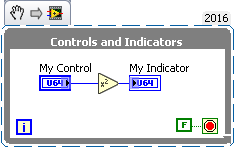
\includegraphics{images/fpga_labview.png}

Hardwarebeschleunigter LabView Code

Durch dieses Konzept kann ein bereits bestehender Python-Code sehr
leicht durch Hardwarebeschleunigung erweitert werden. Statt komplexe
Funktionen auszuführen, können die Daten an das FPGA gesendet und die
Resultate im Anschluss gelesen werden. Zeitunkritische Aufgaben, wie das
Senden von Daten über an andere Rechner im Netzwerk, das Anpassen von
Parametern oder die Darstellung der Daten kann weiterhin vom
Python-Programm übernommen werden und müssen so nicht noch einmal neu
entwickelt werden.

    \hypertarget{xilinx-pynq}{%
\subsection{Xilinx PYNQ}\label{xilinx-pynq}}

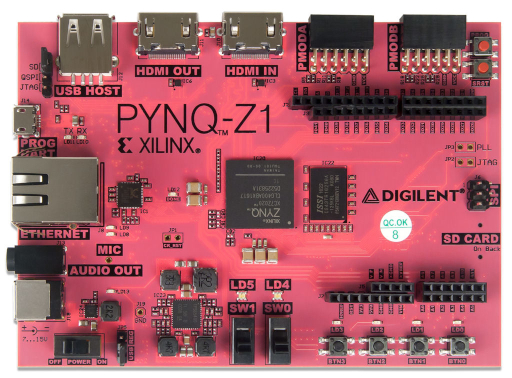
\includegraphics{images/fpga_pynq.jpg}

Quelle Bild:
https://shop.trenz-electronic.de/media/image/47/bb/33/29034\_1.jpg

Ein weiteres interessantes Python / FPGA Konzept kommt direkt von
\emph{Xilinx}. Xilinx ist der führende Hersteller für FPGA-Chips und ist
somit im Bereich des high-speed-DSP sehr weit verbreitet. Im Projekt
\emph{PYNQ} werden Boards direkt mit Python programmiert. Daten werden
via Overlays bis zum FPGA übertragen und werden dort in der Hardware
verarbeitet. Aktuell gibt es noch sehr wenige Boards, die dieses Konzept
unterstützen. Diese reichen aber vom
\href{https://store.digilentinc.com/pynq-z1-python-productivity-for-zynq-7000-arm-fpga-soc/}{unteren
Preissegment} bis in den
\href{https://www.xilinx.com/products/boards-and-kits/zcu111.html\#overview}{professionellen
Bereich}. Auch hier ist leider keines der Boards im Besitz der Gruppe.
Die Informationen stammen entsprechend von der
\href{http://www.pynq.io/}{Website} und dem
\href{https://pynq.readthedocs.io/en/latest/index.html}{Getting Started}
zu dieser Plattform.

Sehr interessant ist das Entwicklungskonzept der Software. Die benötigte
Software - u.a. Jupyter Notebook - auf eine SD-Karte gespielt und Board
via LAN mit dem Rechner verbunden. Dabei ist es egal, ob eine direkte
Verbindung besteht oder das PYNQ an den Router im Netzwerk angeschlossen
wird. Über den Webbrowser wird anschließen auf das Board zugegriffen.
Die gesamte Softwareentwicklung findet anschließend in Jupyter Notebook
statt und kann direkt auf dem Board ausgeführt werden. Auf dem
Entwicklungsrechner muss somit keine zusätzliche Software installiert
werden. Benötigte Dateien werden via
\href{https://www.samba.org/}{Samba} zwischen den Geräten ausgetauscht.

Auch dieses Konzept ermöglicht eine schnelle Umsetzung der
Hardwarebeschleunigung in Python. Durch die Verfügbarkeit von günstigen
Boards eignet sich PYNQ auch sehr gut für den privaten Bereich.

    \hypertarget{fazit}{%
\section{Fazit}\label{fazit}}

Digitale Signalverarbeitung in Python ist durch Unterstützung der
Bibliotheken von \emph{NumPy}, \emph{SciPy} und \emph{Matplotlib} ohne
weiteres möglich. Die Entwicklung in \emph{Octave} ist dabei immer noch
etwas einfacher, lässt aber die Flexibilität von \emph{Python}
vermissen. Dennoch bietet \emph{Python} neben der bekannten schnellen
Code Entwicklung durch die optimierten Bibliotheken eine beeindruckende
Geschwindigkeit, ohne dass der Code extra optimiert werden muss. Einzig
die Hardwareunterstützung durch FPGAs ist nicht weit verbreitet, aber
dennoch möglich. Auch hier mit einem beeindruckend geringem
Entwicklungsaufwand. Projekte im Bereich DSP können so sehr schnell
entwickelt und erprobt werden.

    \hypertarget{quellen}{%
\section{Quellen}\label{quellen}}

\begin{itemize}
\tightlist
\item
  https://www.scipy.org/
\item
  https://numpy.org/
\item
  https://matplotlib.org/
\item
  https://www.geeksforgeeks.org/python-lists-vs-numpy-arrays/
\item
  https://matplotlib.org/mpl\_toolkits/mplot3d/tutorial.html
\item
  https://nifpga-python.readthedocs.io/en/latest/index.html
\item
  http://www.pynq.io/
\end{itemize}


    % Add a bibliography block to the postdoc
    
    
    
\end{document}
